% ============================================================================
%  Doc T -- SPEAR3 Legacy LLRF: Tuner Control System Technical Analysis
%  Build:  powershell -ExecutionPolicy Bypass -File build.ps1 -Doc T
%  Engine: LuaLaTeX (required -- see the Unicode note in preamble.tex)
% ============================================================================
\documentclass[letterpaper,11pt]{article}
% ============================================================================
%  SPEAR3 RF System documentation -- shared preamble
%  Engine: LuaLaTeX.  Build with build.ps1 (latexmk -lualatex).
% ============================================================================

\usepackage[letterpaper,top=1in,bottom=1in,left=1.05in,right=1.05in]{geometry}

% --- fonts -----------------------------------------------------------------
\usepackage{fontspec}
\setmainfont{TeX Gyre Termes}
\setsansfont{TeX Gyre Heros}
\setmonofont{Consolas}[Scale=0.86]

% --- Unicode safety --------------------------------------------------------
% LuaLaTeX DROPS unmapped glyphs SILENTLY -- an unmapped U+03BC turns "8 uF"
% into "8 F".  Every non-ASCII character used in these documents is mapped
% here.  The build script fails if the log reports "Missing character".
\usepackage{newunicodechar}
\newunicodechar{μ}{\ensuremath{\mu}}      \newunicodechar{µ}{\ensuremath{\mu}}
\newunicodechar{Ω}{\ensuremath{\Omega}}   \newunicodechar{≈}{\ensuremath{\approx}}
\newunicodechar{≥}{\ensuremath{\geq}}     \newunicodechar{≤}{\ensuremath{\leq}}
\newunicodechar{≠}{\ensuremath{\neq}}     \newunicodechar{×}{\ensuremath{\times}}
\newunicodechar{÷}{\ensuremath{\div}}     \newunicodechar{±}{\ensuremath{\pm}}
\newunicodechar{−}{\ensuremath{-}}        \newunicodechar{√}{\ensuremath{\sqrt{}}}
\newunicodechar{α}{\ensuremath{\alpha}}   \newunicodechar{β}{\ensuremath{\beta}}
\newunicodechar{φ}{\ensuremath{\varphi}}  \newunicodechar{ω}{\ensuremath{\omega}}
\newunicodechar{Δ}{\ensuremath{\Delta}}   \newunicodechar{τ}{\ensuremath{\tau}}
\newunicodechar{θ}{\ensuremath{\theta}}   \newunicodechar{λ}{\ensuremath{\lambda}}
\newunicodechar{π}{\ensuremath{\pi}}      \newunicodechar{σ}{\ensuremath{\sigma}}
\newunicodechar{₀}{\ensuremath{_0}}       \newunicodechar{₁}{\ensuremath{_1}}
\newunicodechar{₂}{\ensuremath{_2}}       \newunicodechar{²}{\ensuremath{^2}}
\newunicodechar{³}{\ensuremath{^3}}       \newunicodechar{⁴}{\ensuremath{^4}}
\newunicodechar{⁻}{\ensuremath{^-}}       \newunicodechar{⁺}{\ensuremath{^+}}
\newunicodechar{→}{\ensuremath{\rightarrow}}
\newunicodechar{←}{\ensuremath{\leftarrow}}
\newunicodechar{↔}{\ensuremath{\leftrightarrow}}
\newunicodechar{⇒}{\ensuremath{\Rightarrow}}
\newunicodechar{⊕}{\ensuremath{\oplus}}   \newunicodechar{∥}{\ensuremath{\parallel}}
\newunicodechar{°}{\ensuremath{^\circ}}   \newunicodechar{·}{\ensuremath{\cdot}}
\newunicodechar{≪}{\ensuremath{\ll}}      \newunicodechar{≫}{\ensuremath{\gg}}
\newunicodechar{✓}{\checkmark}            \newunicodechar{⚠}{\textbf{!}}
\newunicodechar{–}{--}                    \newunicodechar{—}{---}

% --- maths and units -------------------------------------------------------
\usepackage{amsmath,amssymb}
\usepackage{siunitx}
\DeclareSIUnit\voltampere{VA}
\DeclareSIUnit\VAR{var}
% range-phrase must not rely on literal spaces (LaTeX strips them from a key
% value, so "{ to }" renders as "10to20") and must force text mode (siunitx
% sets numbers in math, where a bare "--" becomes two minus signs).
\sisetup{per-mode=symbol,range-phrase={\text{--}},range-units=single,
         group-minimum-digits=4,detect-weight=true}

% --- tables ----------------------------------------------------------------
\usepackage{longtable,booktabs,array,tabularx,multirow}
\usepackage{ragged2e}
\setlength{\LTleft}{0pt}\setlength{\LTright}{0pt}
\renewcommand{\arraystretch}{1.18}
% left-aligned, hyphenating paragraph column used by every wide table
\newcolumntype{P}[1]{>{\RaggedRight\arraybackslash}p{#1}}
% Same, but \small: for dense tables.  The size must live in the column type --
% wrapping a longtable in {\small ...} breaks its page-breaking \write.
\newcolumntype{Q}[1]{>{\small\RaggedRight\arraybackslash}p{#1}}

% --- graphics and figures --------------------------------------------------
\usepackage{graphicx}
% Resolved from the document's own folder, which is the working directory.
\graphicspath{{../common/}{../common/photos/}{../common/generated/}}
\usepackage{float}
\usepackage[font=small,labelfont=bf,width=0.92\linewidth]{caption}
\usepackage{comment}

% A figure must not drift out of the section it belongs to.  With 47 floats
% LaTeX will otherwise push them pages away from the text that discusses them.
\usepackage[section]{placeins}

% Default float parameters are tuned for papers with two or three figures.
% This document is figure-dense, so allow more of a page to be float and more
% floats per page; without this, figures queue up and drift several pages.
\renewcommand{\topfraction}{0.88}
\renewcommand{\bottomfraction}{0.70}
\renewcommand{\textfraction}{0.10}
\renewcommand{\floatpagefraction}{0.72}
\setcounter{topnumber}{3}
\setcounter{bottomnumber}{2}
\setcounter{totalnumber}{5}

% Image size policy.  Photographs are capped in BOTH width and height so that
% no figure can ever exceed roughly half a page, whatever its aspect ratio.
\newlength{\photomaxh}\setlength{\photomaxh}{0.34\textheight} % ~1/3 page
\newlength{\widemaxh} \setlength{\widemaxh}{0.46\textheight}  % ~1/2 page

% \photofig{file}{caption}{label}      -- default, about 1/3 page
\newcommand{\photofig}[3]{%
  \begin{figure}[htbp]\centering
    \includegraphics[width=0.62\linewidth,height=\photomaxh,keepaspectratio]{#1}%
    \caption{#2}\label{#3}
  \end{figure}}
% \widefig{file}{caption}{label}       -- for detailed schematics, about 1/2 page
\newcommand{\widefig}[3]{%
  \begin{figure}[htbp]\centering
    \includegraphics[width=0.94\linewidth,height=\widemaxh,keepaspectratio]{#1}%
    \caption{#2}\label{#3}
  \end{figure}}
% \smallfig{file}{caption}{label}      -- for low-resolution sources
\newcommand{\smallfig}[3]{%
  \begin{figure}[htbp]\centering
    \includegraphics[width=0.44\linewidth,height=0.26\textheight,keepaspectratio]{#1}%
    \caption{#2}\label{#3}
  \end{figure}}
% \tallfig{file}{caption}{label}       -- portrait-orientation photographs.
% A tall photo capped at \photomaxh comes out only ~45 mm wide, so these are
% capped by height instead and allowed a narrower column.
\newcommand{\tallfig}[3]{%
  \begin{figure}[tbp]\centering
    \includegraphics[width=0.46\linewidth,height=0.50\textheight,keepaspectratio]{#1}%
    \caption{#2}\label{#3}
  \end{figure}}
% two portrait photographs side by side under one caption:
% \tallpairfig{fileA}{subA}{labA}{fileB}{subB}{labB}{caption}{label}
\newcommand{\tallpairfig}[8]{%
  \begin{figure}[tbp]\centering
    \begin{minipage}[b]{0.46\linewidth}\centering
      \includegraphics[width=\linewidth,height=0.40\textheight,keepaspectratio]{#1}%
      \subcaption{#2}\label{#3}
    \end{minipage}\hfill
    \begin{minipage}[b]{0.46\linewidth}\centering
      \includegraphics[width=\linewidth,height=0.40\textheight,keepaspectratio]{#4}%
      \subcaption{#5}\label{#6}
    \end{minipage}
    \caption{#7}\label{#8}
  \end{figure}}
% two photographs side by side, each about 1/4 page
\newcommand{\pairfig}[6]{%
  \begin{figure}[htbp]\centering
    \begin{minipage}[t]{0.48\linewidth}\centering
      \includegraphics[width=\linewidth,height=0.26\textheight,keepaspectratio]{#1}%
      \subcaption{#2}\label{#3}
    \end{minipage}\hfill
    \begin{minipage}[t]{0.48\linewidth}\centering
      \includegraphics[width=\linewidth,height=0.26\textheight,keepaspectratio]{#4}%
      \subcaption{#5}\label{#6}
    \end{minipage}
  \end{figure}}
\usepackage{subcaption}

% --- diagrams --------------------------------------------------------------
\usepackage{tikz}
\usetikzlibrary{arrows.meta,positioning,fit,backgrounds,calc,shapes.geometric,
                shapes.misc,chains,decorations.pathreplacing,patterns,matrix}
\usepackage{pgfplots}\pgfplotsset{compat=1.18}
\usepackage{rotating}                  % sidewaysfigure, if a portrait page is wanted
\usepackage{pdflscape}                 % landscape: rotates the PAGE in the PDF
\usepackage[export]{adjustbox}         % max width= / max height= on a box

% Shrink a diagram to the text width only if it would otherwise overflow, so
% figures drawn at their natural scale are never enlarged or needlessly shrunk.
\newsavebox{\fitbox}
\newenvironment{fitpicture}
  {\begin{lrbox}{\fitbox}}
  {\end{lrbox}%
   \ifdim\wd\fitbox>\linewidth
     \resizebox{\linewidth}{!}{\usebox{\fitbox}}%
   \else
     \usebox{\fitbox}%
   \fi}

% House diagram style.  Keep every block diagram in these styles so the
% document reads as one drawing set rather than a scrapbook.
\definecolor{cCtrl}{HTML}{1F4E79}   % control / EPICS
\definecolor{cPlc} {HTML}{7F6000}   % PLC / interlock
\definecolor{cPwr} {HTML}{843C0C}   % high power
\definecolor{cRf}  {HTML}{2E6B34}   % RF signal path
\definecolor{cNeut}{HTML}{3B3B3B}
\tikzset{
  blk/.style   ={draw=cNeut,fill=white,rounded corners=1.6pt,align=center,
                 inner sep=4pt,font=\scriptsize,minimum height=8mm},
  ctrl/.style  ={blk,draw=cCtrl,fill=cCtrl!7,text=cCtrl!85!black},
  plc/.style   ={blk,draw=cPlc, fill=cPlc!8, text=cPlc!80!black},
  pwr/.style   ={blk,draw=cPwr, fill=cPwr!7, text=cPwr!85!black},
  rf/.style    ={blk,draw=cRf,  fill=cRf!7,  text=cRf!80!black},
  grp/.style   ={draw=black!35,dashed,rounded corners=3pt,inner sep=7pt},
  lbl/.style   ={font=\scriptsize\itshape,text=black!62},
  sig/.style   ={-{Stealth[length=2.2mm]},draw=cNeut,thick},
  fib/.style   ={sig,densely dashed},
  bus/.style   ={draw=cNeut,line width=1.1pt},
  tag/.style   ={font=\tiny,inner sep=1.4pt,fill=white,text=black!70},
}
% consistent caption for a TikZ figure
\newcommand{\diagcap}[2]{\caption{#1}\label{#2}}

% --- lists, misc -----------------------------------------------------------
\usepackage{enumitem}
\setlist{nosep,leftmargin=1.35em}
\providecommand{\tightlist}{%   emitted by pandoc for compact lists
  \setlength{\itemsep}{0pt}\setlength{\parskip}{0pt}}
\usepackage[table]{xcolor}
\usepackage{soul}
\usepackage{microtype}
\usepackage{fancyhdr}
\usepackage{lastpage}
\usepackage{needspace}

% --- callout box for warnings / key findings -------------------------------
\usepackage[most]{tcolorbox}
\newtcolorbox{keynote}[1][]{colback=black!3,colframe=black!45,boxrule=0.4pt,
  arc=1.5pt,left=5pt,right=5pt,top=4pt,bottom=4pt,fontupper=\small,#1}
\newtcolorbox{warnbox}[1][]{colback=cPwr!5,colframe=cPwr!70,boxrule=0.7pt,
  arc=1.5pt,left=5pt,right=5pt,top=4pt,bottom=4pt,fontupper=\small,#1}

% --- cross references and links --------------------------------------------
\usepackage[hyphens]{url}
\usepackage[hidelinks,pdfusetitle,bookmarksnumbered]{hyperref}
\usepackage[capitalise,nameinlink]{cleveref}
\crefname{section}{\S}{\S\S}
\Crefname{section}{Section}{Sections}
% Spell out "Figure" for \cref too; cleveref's default abbreviates it to "Fig.",
% which reads inconsistently beside \Cref in the same sentence.
\crefname{figure}{Figure}{Figures}
% Lowercase \cref on a section prints "§5.7" / "§§10.2--10.5" -- no space after
% the sign and an en-dash range, matching the hand-written style it replaced.
\crefformat{section}{\S#2#1#3}
\crefrangeformat{section}{\S\S#3#1#4--#5#2#6}
\crefmultiformat{section}{\S#2#1#3}{ and~\S#2#1#3}{, \S#2#1#3}{ and~\S#2#1#3}

% Repository paths are long and unhyphenatable; allow breaks after / and .
% Long file paths and CamelCase document names have no natural break points, so
% url's default break set is not enough: allow a break before any capital and
% after the usual separators.
\newcommand{\fpath}[1]{{\ttfamily\small\Urlmuskip=0mu plus 1mu\relax
  \def\UrlBreaks{\do\/\do\.\do\-\do\_\do\:\do\A\do\B\do\C\do\D\do\E\do\F\do\G
    \do\H\do\I\do\J\do\K\do\L\do\M\do\N\do\O\do\P\do\Q\do\R\do\S\do\T\do\U
    \do\V\do\W\do\X\do\Y\do\Z}%
  \urlstyle{tt}\nolinkurl{#1}}}
\setlength{\emergencystretch}{2em}

% --- headers ---------------------------------------------------------------
\pagestyle{fancy}\fancyhf{}
\renewcommand{\headrulewidth}{0.3pt}
\fancyhead[L]{\footnotesize\nouppercase{\rightmark}}
\fancyhead[R]{\footnotesize\thepage\ / \pageref{LastPage}}
\renewcommand{\sectionmark}[1]{\markright{\thesection\quad #1}}
\fancypagestyle{plain}{\fancyhf{}\renewcommand{\headrulewidth}{0pt}%
  \fancyfoot[C]{\footnotesize\thepage}}

\setcounter{tocdepth}{2}
\setcounter{secnumdepth}{3}


% Equations are numbered within sections, as in Doc P.
\numberwithin{equation}{section}

% Verbatim-ish blocks.  \sigblock keeps the column alignment of signal and PV
% traces; \codeblock is for C, EPICS database and SNL excerpts.
\usepackage{fancyvrb}
\DefineVerbatimEnvironment{sigblock}{Verbatim}%
  {fontsize=\footnotesize,frame=leftline,framerule=0.6pt,rulecolor=\color{cNeut!35},
   framesep=6pt,xleftmargin=8pt}
\DefineVerbatimEnvironment{codeblock}{Verbatim}%
  {fontsize=\footnotesize,frame=leftline,framerule=0.6pt,rulecolor=\color{cCtrl!45},
   framesep=6pt,xleftmargin=8pt}

% --- [Rn] citation scheme --------------------------------------------------
% Doc T uses the same numbered [Rn] reference list as Doc L and Doc I, so that a
% source cited in one document carries the same style of tag in all of them.
% \R{n} links to the defining row in the source index; \RDEF{n} is that row.
% The anchor is wrapped in a zero-size raisebox: a bare \hypertarget occupies a
% line box and pushes the visible tag down a line inside a p{} cell.
\DeclareRobustCommand{\R}[1]{\hyperlink{ref:R#1}{[R#1]}}
\DeclareRobustCommand{\RDEF}[1]{%
  \raisebox{0pt}[0pt][0pt]{\hypertarget{ref:R#1}{}}\textbf{[R#1]}}

% --- open items ------------------------------------------------------------
% \openitem{On} tags the statement in the body that is still unverified and
% links forward to the Open Items table; \openpage{On} is the table's back-link.
\DeclareRobustCommand{\openitem}[1]{\,%
  \raisebox{0pt}[0pt][0pt]{\hypertarget{open:#1}{}}\label{openp:#1}%
  \hyperlink{openitems}{\textcolor{cPlc}{\bfseries\scriptsize[#1]}}}
\newcommand{\openpage}[1]{\hyperlink{open:#1}{p.~\pageref*{openp:#1}}}

\hypersetup{pdftitle={SPEAR3 Legacy LLRF: Tuner Control System Technical Analysis},
  pdfauthor={Faya Wang},pdfsubject={Doc T R0 - Draft}}

\title{\vspace{-1.4cm}\bfseries SPEAR3 Legacy LLRF\\[2mm]
       \Large Tuner Control System Technical Analysis}
\author{}
\date{}

\begin{document}
\maketitle
\thispagestyle{plain}

\begin{center}
\begin{minipage}{0.86\linewidth}\small
\begin{tabular}{@{}ll@{}}
\textbf{Document ID} & Doc T \\
\textbf{Revision}    & R0 \\
\textbf{Status}      & Draft \\
\textbf{Author}      & Faya Wang \\
\textbf{Reviewer}    & Jim Sebek and others \\
\textbf{Classification} & Tier 2 --- Legacy Tuner Control Reference \\
\textbf{Affiliation} & SSRL, SLAC National Accelerator Laboratory \\
\textbf{Date}        & 30 September 2026 \\
\end{tabular}
\end{minipage}
\end{center}

\vspace{4mm}
\begin{keynote}
This document reverse-engineers the mechanical cavity tuner loop \emph{as
deployed on SPEAR3}, from the legacy \fpath{spear-rf-code-legacy/rfApp/} source
tree. Two things are easy to get wrong when reading it. First, the architecture
is a dual loop, but only the inner phase-regulation loop is active on SPEAR3:
the outer voltage loop is PEP-II inheritance and its phase offset is fixed at
zero. Second, the \textbf{AB 1746-HSTP1 is still the in-service controller};
the Galil DMC-4143 is in development and goes online only when the LLRF upgrade
completes. The \hyperref[sec:open-items]{Open Items} register lists the points
that still require field verification.
\end{keynote}

\clearpage
\tableofcontents
\clearpage
\listoffigures
\clearpage

% !TeX root = T_tuner_control_analysis.tex
% Generated from T_TUNER_CONTROL_SYSTEM_ANALYSIS.md by scripts/md2tex.js, then hand-corrected.
% Edit THIS file, not the markdown.

\section*{Open Items}\label{sec:open-items}
\hypertarget{openitems}{}
\addcontentsline{toc}{section}{Open Items}
\markboth{Open Items}{Open Items}

Each entry below is a statement in this document that rests on an operator
screen, a vendor note or an undocumented convention rather than on a file in
the repository. The page link returns to the statement.

\begin{longtable}[]{@{}Q{\dimexpr 0.0520\linewidth-1.60\tabcolsep\relax}Q{\dimexpr 0.3000\linewidth-1.60\tabcolsep\relax}Q{\dimexpr 0.3200\linewidth-1.60\tabcolsep\relax}Q{\dimexpr 0.2080\linewidth-1.60\tabcolsep\relax}Q{\dimexpr 0.1200\linewidth-1.60\tabcolsep\relax}@{}}
\toprule\noalign{}
ID & Item & Required evidence & Needed before & Page \\
\midrule\noalign{}
\endhead
\bottomrule\noalign{}
\endlastfoot
O1 & The \textbf{Tuner Inputs \& Constants} operator panel is the only stated source for the nominal values of every parameter that is commented out in the database source. & Archive the screen file (or an equivalent configuration export) in the repository, and record which values autosave actually restores on the running IOC. & Any claim that the tuner is functional as configured & \openpage{O1} \\
O2 & The mm-per-degree conversion is quoted as a \textbf{range}, 0.020--0.030 mm/\textdegree, not a single commissioned number. & The per-cavity commissioned value, or the measurement that established the range. & Quantitative loop-gain analysis & \openpage{O2} \\
O3 & The \textbf{IQA phase calibration} that defines the zero of \texttt{LOAD:ANGLE:ERR} has no recorded procedure or last-performed date. & A written calibration procedure and the date it was last run on each cavity. & Trusting that \texttt{ERR}~=~0 means resonance & \openpage{O3} \\
O4 & Whether \textbf{autosave} is actually enabled for the tuner parameter set on the production IOC. & The autosave request file list and a restart test. & Any statement about behavior after an IOC restart & \openpage{O4} \\
O5 & The \textbf{loop gain} \texttt{CAVTUNR:LOOP:GAIN} is stated to run at unity, but the value is operator-settable and not archived. & The as-running value, read from the live IOC. & Reproducing the loop bandwidth figures & \openpage{O5} \\
O6 & \textbf{Mechanical condition} of the tuner mechanisms. The 2023 inspection recorded bellows and limit-switch problems on three cavities. & A current inspection, and whether the recorded faults were repaired. & Assuming the full $-29.5$ to $+18$ mm travel is usable & \openpage{O6} \\
O7 & The \textbf{Galil DMC-4143} replacement has test moves recorded but no commissioning record or cutover plan. & A commissioning test report and the cutover criteria. & Scheduling the controller swap & \openpage{O7} \\
O8 & The inner-loop gain \cref{eq:geff} reuses the \emph{park}-mode degrees-per-kHz constant \texttt{0.00004726891}, which differs from the physical load-angle conversion by about a factor of five. & Confirmation of which conversion the inner loop is correctly analyzed with, ideally from a measured step response. & Any quantitative stability margin & \openpage{O8} \\
\end{longtable}

\begin{center}\rule{0.5\linewidth}{0.5pt}\end{center}

\part{What and Why}

\section{Executive Summary}\label{sec:summary}


The SPEAR3 tuner control system keeps each cavity at its resonant frequency by mechanically adjusting a tuner plunger in response to measured phase error. The primary disturbance it compensates is \textbf{beam-loading-induced detuning} --- the reactive component of beam current shifts the cavity's apparent resonant frequency in proportion to beam current. A secondary, slower disturbance is thermal drift from RF heating.

The system was designed as \textbf{two nested feedback loops}:

\begin{longtable}[]{@{}Q{\dimexpr 0.0568\linewidth-1.60\tabcolsep\relax}Q{\dimexpr 0.3295\linewidth-1.60\tabcolsep\relax}Q{\dimexpr 0.3523\linewidth-1.60\tabcolsep\relax}Q{\dimexpr 0.0455\linewidth-1.60\tabcolsep\relax}Q{\dimexpr 0.2159\linewidth-1.60\tabcolsep\relax}@{}}
\toprule\noalign{}
Loop & What it regulates & Controller type & Rate & Status in SPEAR3 \\
\midrule\noalign{}
\endhead
\bottomrule\noalign{}
\endlastfoot
\textbf{Inner} & Phase error (probe − forward) & Proportional → stepper motor & \qty{0.5}{\hertz} & \textbf{Active} \\
\textbf{Outer} & Cavity voltage (strength) & Leaky integrator → phase offset & \qty{0.5}{\hertz} & \textbf{Disabled by default} \\
\end{longtable}

\textbf{In SPEAR3 as deployed, only the inner loop is active.} It drives the cavity to the resonant frequency calibrated during a no-beam reference procedure. The outer voltage loop exists in the code but its output is structurally clamped to zero (see \cref{sec:outer-total}). The PARK mode frequency-domain path is PEP-II functionality, permanently disabled.

\textbf{Key numbers:}

\begin{itemize}
\tightlist
\item
  \qty{0.5}{\hertz} loop rate (one cycle every \qty{2}{\second}), 4 cavities, station prefix \texttt{SRF1:}
\item
  Stepper motor: 3.81 mm/s, 0.003175 mm/step, range −29.5 to +18 mm
\item
  Phase deadband: 0.25° (design), conversion: 0.020--0.030 mm/° (nominal operational range per \R{15})\openitem{O2}, max delta: 1 mm/cycle
\end{itemize}

\begin{center}\rule{0.5\linewidth}{0.5pt}\end{center}

\section{Physics: Cavity Detuning and Beam Loading}\label{sec:physics}

\emph{Sources}: \R{18}.


\subsection{Why the Tuner Exists}\label{sec:why-tuner}


An RF cavity has a resonant frequency \(f_0\) determined by its geometry. When driven off-resonance, the generator must supply extra reactive power. The mechanical tuner adjusts cavity geometry to keep \(f_0\) aligned with the drive frequency (476 MHz at SPEAR3), minimizing reflected power and maximizing efficiency.

Two phenomena shift the effective resonant frequency during operation:

\textbf{Beam loading (primary, fast):} When stored beam traverses the cavity, the reactive component of the beam-induced current shifts the apparent resonant frequency by:

\begin{equation}\label{eq:detune-beam}
  \Delta f_{beam} = -\frac{f_0}{2}\cdot\frac{R}{Q}\cdot\frac{I_{b1}\sin\phi_s}{V_{gap}}
\end{equation}

where \(I_{b1} = 2 I_b\) is the \emph{fundamental} component of the bunched beam current (\(I_b\) being the DC average), \(\phi_s\) is synchronous phase, \(R/Q \approx \qty{117}{\ohm}\) is the cavity geometric shunt-impedance ratio, and \(V_{gap}\) is gap voltage. Because \(R/Q\) depends only on cavity geometry, \cref{eq:detune-beam} is independent of \(Q_L\) and of the coupling factor; the equivalent loaded form is \(\Delta f_{beam} = -(f_0/2Q_L)\,I_{b1}R_L\sin\phi_s/V_{gap}\) with \(R_L = R_s/(1+\beta)\) and \(Q_L \approx 7000\). This detuning is proportional to beam current and changes dynamically as beam is injected, decays, or is lost. At SPEAR3 operating conditions (\(I_b \sim 100\text{–}500\) mA) beam loading detunes the cavity by tens of kHz --- about \qty{-36}{\kilo\hertz} at \qty{500}{\milli\ampere}.

\textbf{Thermal drift (secondary, slow):} RF heating causes slow mechanical deformation of the cavity body, shifting the resonant frequency on timescales of minutes to hours. At SPEAR3's operating gradient this is much smaller than beam loading.

\subsection{The Load Angle}\label{sec:load-angle}


For a driven cavity with beam loading, define:

\begin{itemize}
\tightlist
\item
  \(\phi_L\) = load angle = phase of cavity field relative to generator
\item
  \(\psi\) = forward coupler phase relative to cavity probe
\end{itemize}

The optimal detuning \(\Delta\omega_{opt}\) for minimum generator power is the same quantity expressed in angular frequency:

\begin{equation}\label{eq:detune-opt}
  \Delta\omega_{opt} = -\frac{\omega_0}{2Q_L} \cdot \frac{I_{b1} R_L \sin\phi_s}{V_{gap}}
\end{equation}

This corresponds to a target load angle \(\psi_{target}\) where the generator operates most efficiently; for SPEAR3 at \qty{500}{\milli\ampere} that target is \(\psi_{L} \approx \qty{-46}{\degree}\) (Doc~P).

\subsection{How the Error Signal Maps to Detuning}\label{sec:error-to-detuning}


The inner loop measures:

\begin{equation}\label{eq:error-def}
  \text{error} = \phi_{probe} - \phi_{fwd} + \theta_{offset}
\end{equation}

In \cref{eq:error-def}, with \(\theta_{offset} = 0\) (as in SPEAR3), \texttt{error\ =\ 0} means \(\phi_{probe} = \phi_{fwd}\), which corresponds to \textbf{resonance} (zero detuning). The tuner drives toward this condition.

With a nonzero \(\theta_{offset}\), the tuner drives to \(\phi_{probe} - \phi_{fwd} = -\theta_{offset}\), applying a deliberate detuning. The exact relation is \(\tan\psi_L = 2Q_L\,\Delta f/f_0\), so for the small angles the loop actually works over:

\begin{equation}\label{eq:theta-to-df}
  \Delta f \approx \frac{f_0}{2 Q_L}\cdot\frac{\pi\,\theta}{180°}
  \qquad\text{i.e.}\qquad \Delta f \approx \frac{f_0\,\theta}{114.6\,Q_L}
\end{equation}

At \(Q_L \approx 7000\) this is about \qty{0.6}{\kilo\hertz} per degree of load angle.

\subsection{The IQA Calibration Requirement --- Why the Target Is Zero}\label{sec:iqa-calibration}


The inner loop drives \texttt{LOAD:\allowbreak{}ANGLE:\allowbreak{}ERR\ →\ 0}. But the raw IQA measurements include arbitrary phase offsets from cable lengths, directional coupler geometry, and signal conditioning hardware. The measured phase difference at true resonance is generally \emph{not} zero.

\textbf{A calibration step establishes the zero reference:}

\begin{enumerate}
\def\labelenumi{\arabic{enumi}.}
\tightlist
\item
  With \textbf{no beam} (so beam loading does not shift the resonant frequency), operators sweep the tuner through resonance
\item
  At resonance (confirmed by minimum reflected power or maximum stored energy), the EPICS IQA phase offset parameters are set so that \texttt{PROBE:\allowbreak{}PHASE.\allowbreak{}L\ −\ FRWD:\allowbreak{}PHASE.\allowbreak{}L\ =\allowbreak{}\ 0}
\item
  From that point forward, \texttt{LOAD:\allowbreak{}ANGLE:\allowbreak{}ERR\ =\allowbreak{}\ 0} means resonance; any nonzero value \(\epsilon\) means detuning by \(\Delta f \approx f_0\,\epsilon/(114.6\,Q_L)\) (\cref{eq:theta-to-df})
\end{enumerate}

\textbf{EPICS panel parameters for this calibration:} The per-signal offsets described in step 2 are set via the \textbf{"Probe Phase Offset"} and \textbf{"Frwd Phase Offset"} parameters on the Tuner Inputs \& Constants panel \R{15}. These are the operator-accessible knobs that translate the raw IQA \texttt{.L} measurement to zero at resonance. Both offsets are determined during tuner configuration.

\textbf{Why \texttt{.L} rather than \texttt{.VAL}?} Both \texttt{PROBE:PHASE} and \texttt{FRWD:PHASE} have a \texttt{.VAL} field with an individual per-signal phase offset subtracted (for beam physics applications). The \texttt{.L} field is the raw input before this offset. Using \texttt{.L} means the load angle calibration is set once at the system level (both \texttt{.L} traces zeroed at resonance) rather than needing to track per-signal offsets.

\textbf{Practical implication:} If the IQA phase calibration is incorrect or has drifted (hardware swap, cable re-routing), the tuner drives the cavity to the wrong frequency\openitem{O3} --- it minimizes the measured phase difference, but that measured zero no longer corresponds to the true resonance. The system has no independent check of resonance other than this phase measurement.

\begin{center}\rule{0.5\linewidth}{0.5pt}\end{center}

\section{Dual-Loop Architecture Overview}\label{sec:architecture}

\emph{Sources}: \R{1}, \R{5}, \R{8}, \R{9}, \R{10}, \R{13}.


\subsection{The Two Loops}\label{sec:two-loops}


The system was designed with two nested feedback loops. The \textbf{inner loop} (phase regulation) runs once every \qty{2}{\second} (\qty{0.5}{\hertz}) and drives a stepper motor to null the measured phase error. The \textbf{outer loop} (voltage regulation) is a slow integrator that adjusts the inner loop's phase setpoint to maintain cavity voltage. \Cref{fig:tuner-loops} shows how the two nest.

\begin{figure}[tbp]
\centering
\begin{fitpicture}% !TeX root = ../T_tuner_control_analysis.tex
% The dual-loop tuner architecture.  The outer loop is drawn dashed and greyed
% because on SPEAR3 its output is fixed at zero -- it is PEP-II inheritance.
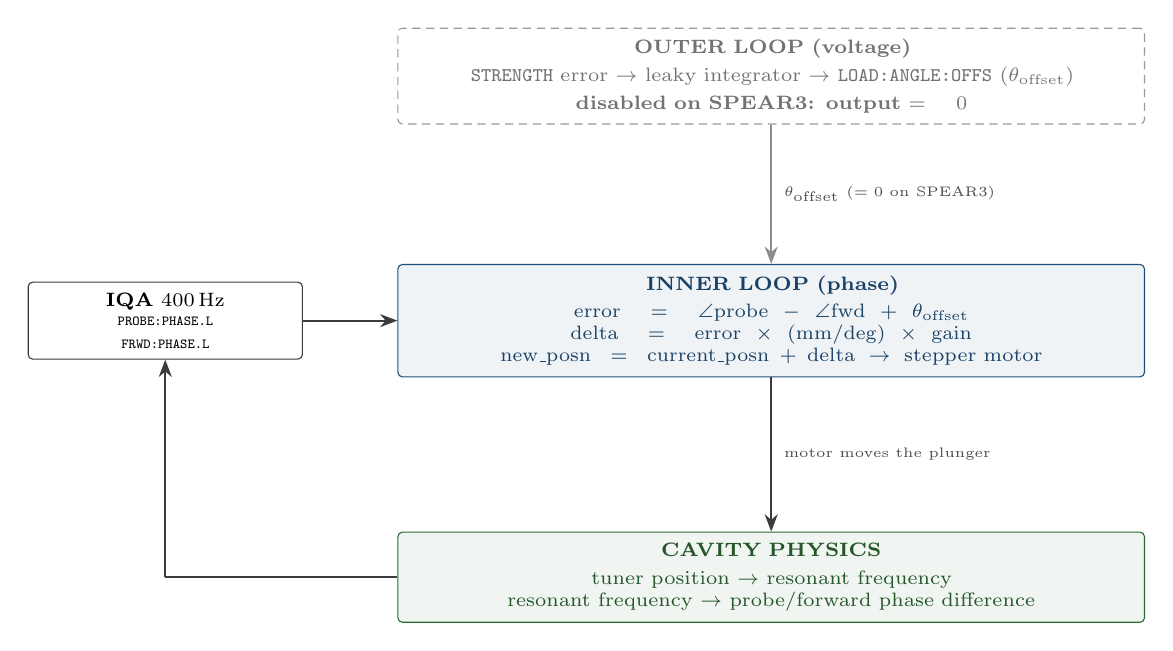
\begin{tikzpicture}[font=\scriptsize, x=1mm, y=1mm]

\node[blk,text width=92mm,anchor=north,draw=black!40,text=black!55,densely dashed]
  (outer) at (60,0)
  {\textbf{OUTER LOOP (voltage)}\\[2pt]
   \texttt{STRENGTH} error $\rightarrow$ leaky integrator
   $\rightarrow$ \texttt{LOAD:ANGLE:OFFS} ($\theta_\text{offset}$)\\[2pt]
   {\bfseries disabled on SPEAR3: output $=0$}};

\node[ctrl,text width=92mm,anchor=north] (inner) at (60,-30)
  {\textbf{INNER LOOP (phase)}\\[2pt]
   $\text{error} = \angle\text{probe} - \angle\text{fwd} + \theta_\text{offset}$\\
   $\text{delta} = \text{error}\times(\text{mm}/\text{deg})\times\text{gain}$\\
   $\text{new\_posn} = \text{current\_posn} + \text{delta}$
   \;$\rightarrow$\; stepper motor};
\draw[sig,draw=black!45] (outer.south) --
  node[right,tag,xshift=1mm]{$\theta_\text{offset}$ ($=0$ on SPEAR3)} (inner.north);

\node[rf,text width=92mm,anchor=north] (phys) at (60,-64)
  {\textbf{CAVITY PHYSICS}\\[2pt]
   tuner position $\rightarrow$ resonant frequency\\
   resonant frequency $\rightarrow$ probe\slash forward phase difference};
\draw[sig] (inner.south) -- node[right,tag,xshift=1mm]{motor moves the plunger} (phys.north);

% the measurement that closes the inner loop.  Placed relative to inner.west so
% the connector between them is exactly horizontal whatever the box heights.
\node[blk,text width=32mm,anchor=east] (iqa) at ($(inner.west)-(12,0)$)
  {\textbf{IQA} \qty{400}{\hertz}\\[1pt]
   {\tiny\texttt{PROBE:PHASE.L}\\ \texttt{FRWD:PHASE.L}}};
\draw[sig] (iqa.east) -- (inner.west);
% plant back to the measurement, entering the IQA from below so that the line
% never crosses the box it is feeding
\draw[draw=cNeut,thick] (phys.west) -- (phys.west -| iqa.south);
\draw[sig] (phys.west -| iqa.south) -- (iqa.south);
\end{tikzpicture}
\end{fitpicture}
\caption{The dual-loop tuner architecture: an inner phase-regulation loop closed on the load angle error, and an outer voltage-regulation loop that biases its setpoint. On SPEAR3 only the inner loop is active.}\label{fig:tuner-loops}
\end{figure}

\textbf{In SPEAR3 as deployed:} \(\theta_{offset} = 0\) always. The outer loop exists in the code architecture but defaults to disabled on a fresh start without autosave (see \cref{sec:outer-total}). In normal operation with autosave restore the outer loop can be functional. The tuner operates in pure resonance-seeking mode --- zero phase error means resonance.

\subsection{Station Configuration}\label{sec:station-config}


\begin{longtable}[]{@{}Q{\dimexpr 0.2368\linewidth-1.33\tabcolsep\relax}Q{\dimexpr 0.4211\linewidth-1.33\tabcolsep\relax}Q{\dimexpr 0.3421\linewidth-1.33\tabcolsep\relax}@{}}
\toprule\noalign{}
Item & Value & Source \\
\midrule\noalign{}
\endhead
\bottomrule\noalign{}
\endlastfoot
Station prefix & \texttt{SRF1:} & \texttt{rf\_\allowbreak{}stn\_\allowbreak{}4CV.\allowbreak{}substitutions,\allowbreak{}v} \\
Cavity prefix & \texttt{\{STN\}:CAV\{N\}} (N=1..4) & \texttt{rf\_cav.db,v} \\
Number of cavities & 4 (independent tuner per cavity) & \texttt{rf\_\allowbreak{}tuner\_\allowbreak{}loop.\allowbreak{}st,\allowbreak{}v} \\
RF frequency & 476 MHz & \texttt{rf\_cav.db,v} \\
Loop rate & \qty{0.5}{\hertz} --- one cycle every \qty{2}{\second} (SCAN="2 second") \R{9} & \texttt{rf\_\allowbreak{}stn\_\allowbreak{}cav.\allowbreak{}db,\allowbreak{}v} \\
\end{longtable}

\subsection{Station State Machine Context}\label{sec:station-state}


The tuner loop only acts in \texttt{ON\_CW} state. The state codes (from \texttt{rf\_\allowbreak{}station\_\allowbreak{}state.\allowbreak{}h,\allowbreak{}v}) are:

\begin{longtable}[]{@{}Q{\dimexpr 0.1111\linewidth-1.33\tabcolsep\relax}Q{\dimexpr 0.0889\linewidth-1.33\tabcolsep\relax}Q{\dimexpr 0.8000\linewidth-1.33\tabcolsep\relax}@{}}
\toprule\noalign{}
State & Code & Tuner Behavior \\
\midrule\noalign{}
\endhead
\bottomrule\noalign{}
\endlastfoot
OFF & 0 & Loop idle, no motor movement \\
PARK & 1 & PEP-II only --- disabled in SPEAR3 \\
TUNE & 2 & Ramp/transition state \\
ON\_FM & 3 & Transition state \\
\textbf{ON\_CW} & \textbf{4} & \textbf{Active control --- phase-domain path} \\
\end{longtable}

\subsection{Software Components}\label{sec:software}


\Cref{fig:signal-chain} shows how the three software layers --- the EPICS database, the SNL state machine and the motor record --- hand the measurement down to the hardware.

\begin{figure}[tbp]
\centering
\begin{fitpicture}% !TeX root = ../T_tuner_control_analysis.tex
% Tuner signal chain across the three software layers: EPICS database, the SNL
% state machine, and the motor record that finally moves hardware.
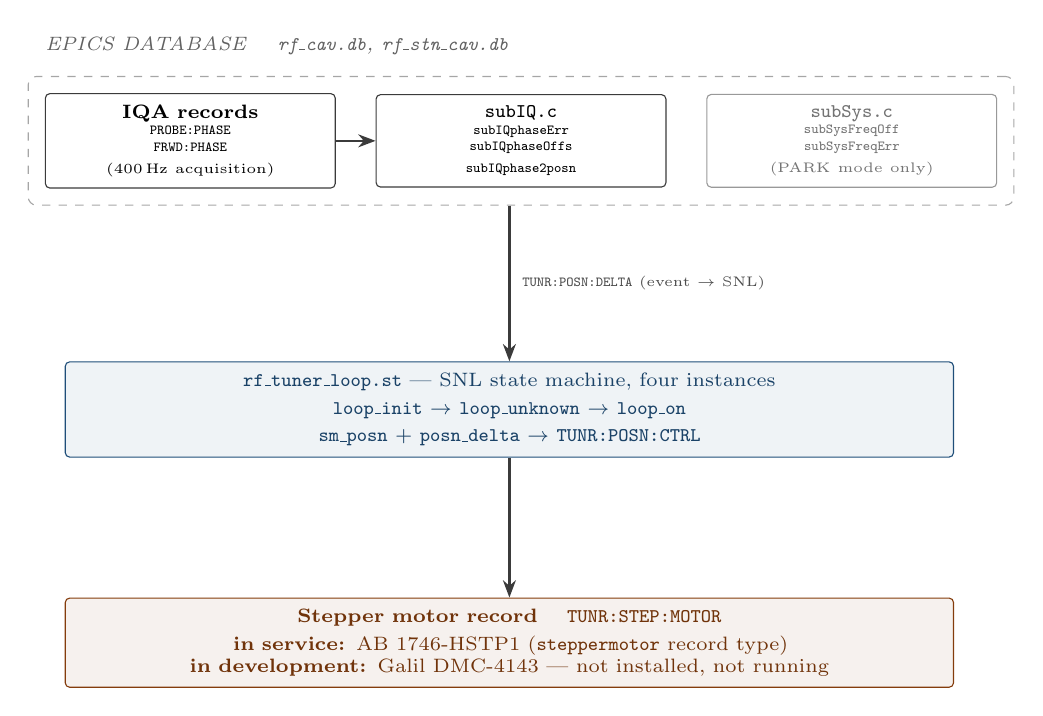
\begin{tikzpicture}[font=\scriptsize, x=1mm, y=1mm]

% ===== EPICS database layer ================================================
\node[blk,text width=34mm,anchor=west] (rec) at (8,0)
  {\textbf{IQA records}\\{\tiny\texttt{PROBE:PHASE}\\ \texttt{FRWD:PHASE}\\ (\qty{400}{\hertz} acquisition)}};
\node[blk,text width=34mm,anchor=west] (iq) at (50,0)
  {\textbf{\texttt{subIQ.c}}\\{\tiny\texttt{subIQphaseErr}\\ \texttt{subIQphaseOffs}\\ \texttt{subIQphase2posn}}};
\node[blk,text width=34mm,anchor=west,draw=black!40,text=black!55] (sys) at (92,0)
  {\textbf{\texttt{subSys.c}}\\{\tiny\texttt{subSysFreqOff}\\ \texttt{subSysFreqErr}\\ (PARK mode only)}};
\draw[sig] (rec.east) -- (iq.west);
\node[grp,fit=(rec)(iq)(sys),inner sep=6pt] (dbbox) {};
\node[lbl,anchor=south west] at ($(dbbox.north west)+(1,1.5)$)
  {EPICS DATABASE \quad\texttt{rf\_cav.db}, \texttt{rf\_stn\_cav.db}};

% ===== SNL layer ===========================================================
\node[ctrl,text width=110mm,anchor=north] (snl) at (67,-28)
  {\textbf{\texttt{rf\_tuner\_loop.st}} --- SNL state machine, four instances\\[2pt]
   \texttt{loop\_init} $\rightarrow$ \texttt{loop\_unknown} $\rightarrow$ \texttt{loop\_on}\\[2pt]
   \texttt{sm\_posn} $+$ \texttt{posn\_delta} $\rightarrow$ \texttt{TUNR:POSN:CTRL}};
% dbbox is a fit node, so its centre is not snl's centre; drop from the point on
% its bottom edge that is directly above snl, or the connector leans.
\draw[sig] (snl.north |- dbbox.south) -- node[right,tag,xshift=1mm]
  {\texttt{TUNR:POSN:DELTA} (event $\rightarrow$ SNL)} (snl.north);

% ===== motor record ========================================================
\node[pwr,text width=110mm,anchor=north] (mot) at (67,-58)
  {\textbf{Stepper motor record} \quad\texttt{TUNR:STEP:MOTOR}\\[2pt]
   \textbf{in service:} AB 1746-HSTP1 (\texttt{steppermotor} record type)\\
   \textbf{in development:} Galil DMC-4143 --- not installed, not running};
\draw[sig] (snl.south) -- (mot.north);
\end{tikzpicture}
\end{fitpicture}
\caption{Tuner signal chain from the cavity probe and forward coupler through the IQA modules to the stepper motor record.}\label{fig:signal-chain}
\end{figure}

\subsubsection{Galil controller status}\label{sec:galil-status}

\begin{warnbox}
Per the system owner: the Galil DMC-4143 control \textbf{has not been installed and is not in operation --- it is in development}. Test moves were performed on the existing cavity motors and worked fine, but the controller is expected to go online only \textbf{when the current LLRF upgrade project is finished}. It has \emph{not} replaced the Allen-Bradley hardware.

\textbf{The AB 1746-HSTP1 stepper controller remains the in-service hardware.} Everything in this document describing present-day tuner behavior refers to the AB path; Galil material is forward-looking.
\end{warnbox}

\begin{center}\rule{0.5\linewidth}{0.5pt}\end{center}

\part{How It Works}

\section{Inner Loop: Phase Regulation}\label{sec:inner-loop}

\emph{Sources}: \R{1}, \R{3}, \R{8}.


This section traces the signal from IQA measurement through to motor command --- the active control path in SPEAR3.

\subsection{Step 1 --- Phase Error Measurement}\label{sec:inner-step1}


\textbf{C function:} \texttt{subIQphaseErr} --- \texttt{rfApp/\allowbreak{}src/\allowbreak{}db/\allowbreak{}subIQ.\allowbreak{}c,\allowbreak{}v} line 566 \R{3}\\
\textbf{EPICS record:} \texttt{\$(S):\allowbreak{}\$(C)LOAD:\allowbreak{}ANGLE:\allowbreak{}ERR}

\begin{codeblock}
psub->val = psub->l = psub->a - psub->b + psub->c + psub->d;
if      (psub->val < -180.0) psub->val += 360.0;
else if (psub->val >  180.0) psub->val -= 360.0;
\end{codeblock}

\begin{equation}\label{eq:load-angle-err}
  \boxed{\text{LOAD:ANGLE:ERR} = \phi_{probe} - \phi_{fwd} + \theta_{offset} + 0}
\end{equation}

\begin{longtable}[]{@{}Q{\dimexpr 0.2958\linewidth-1.33\tabcolsep\relax}Q{\dimexpr 0.2113\linewidth-1.33\tabcolsep\relax}Q{\dimexpr 0.4930\linewidth-1.33\tabcolsep\relax}@{}}
\toprule\noalign{}
Input & PV & Description \\
\midrule\noalign{}
\endhead
\bottomrule\noalign{}
\endlastfoot
INPA (\(\phi_{probe}\)) & \texttt{PROBE:PHASE.L} & Unadjusted probe phase (degrees) \\
INPB (\(\phi_{fwd}\)) & \texttt{FRWD:PHASE.L} & Unadjusted forward phase (degrees) \\
INPC (\(\theta_{offset}\)) & \texttt{LOAD:\allowbreak{}ANGLE:\allowbreak{}OFFS} & Target phase offset (= 0 in SPEAR3) \\
INPD & --- & Spare, always 0 \\
\end{longtable}

Result wrapped to \([-180°, +180°]\). Alarm limits: \texttt{HIHI/\allowbreak{}LOLO\ =\allowbreak{}\ ±5°} (MAJOR).

\textbf{Load angle error limit (Ld Angle Err Limit):} The operator panel exposes a separate parameter \textbf{"Ld Angle Err Limit"} (nominal \textbf{0.5°} per \R{15}) that is distinct from the ±5° EPICS HIHI/LOLO alarms. When \texttt{\textbar{}LOAD:\allowbreak{}ANGLE:\allowbreak{}ERR\textbar{}} exceeds this limit, the outer loading angle offset integrator (\cref{sec:outer-integrator}) is \textbf{frozen} --- no further offset accumulation occurs until the error returns within bounds. This provides a guard against the outer loop winding up during large transient detuning events.

\textbf{Note on \texttt{.L} field:} Uses unadjusted (pre-offset) phase from IQA records. The \texttt{.VAL} field has a per-signal phase offset subtracted for beam physics applications --- that subtraction is separate from the load angle target. See \cref{sec:iqa-calibration} for the calibration requirement that makes \texttt{error\ =\ 0} correspond to resonance.

\begin{codeblock}
grecord(sub,"$(S):$(C)LOAD:ANGLE:ERR") {
    field(INAM,"subIQinit")
    field(SNAM,"subIQphaseErr")
    field(INPA,"$(S):$(C)PROBE:PHASE.L  NPP MS")
    field(INPB,"$(S):$(C)FRWD:PHASE.L   NPP MS")
    field(INPC,"$(S):$(C)LOAD:ANGLE:OFFS.VAL NPP NMS")
    field(EGU,"deg")
    field(HOPR,"10")    field(LOPR,"-10")
    field(HIHI,"5")     field(LOLO,"-5")
    field(HHSV,"MAJOR") field(LLSV,"MAJOR")
}
\end{codeblock}

\subsection{Step 2 --- Phase Error to Position Delta}\label{sec:inner-step2}


\textbf{C function:} \texttt{subIQphase2posn} --- \texttt{rfApp/\allowbreak{}src/\allowbreak{}db/\allowbreak{}subIQ.\allowbreak{}c,\allowbreak{}v} line 586 \R{3}\\
\textbf{EPICS record:} \texttt{\$(S):\allowbreak{}\$(C)TUNR:\allowbreak{}POSN:\allowbreak{}DELTA}

\begin{codeblock}
// Select error source based on station state
if (state == STATION_PARK) error = G;  // park freq error (PEP-II)
else                        error = F;  // load angle error (SPEAR3 ON_CW)

gain = clamp(gain, 0, 1);  // CAVTUNR:LOOP:GAIN

if (|error| > deadband_B):
    delta = clamp(error * C_mm_per_deg * gain, -D_mm, +D_mm)
else:
    delta = 0
\end{codeblock}

\begin{equation}\label{eq:posn-delta}
  \boxed{\Delta x = \text{clamp}\!\left(\epsilon \cdot C_{mm/deg} \cdot G_{loop},\; {-D},\; {+D}\right) \quad \text{if } |\epsilon| > B}
\end{equation}

\begin{longtable}[]{@{}Q{\dimexpr 0.0499\linewidth-1.50\tabcolsep\relax}Q{\dimexpr 0.2639\linewidth-1.50\tabcolsep\relax}Q{\dimexpr 0.5278\linewidth-1.50\tabcolsep\relax}Q{\dimexpr 0.1583\linewidth-1.50\tabcolsep\relax}@{}}
\toprule\noalign{}
Input & PV / Value & Design Value & DB Status \\
\midrule\noalign{}
\endhead
\bottomrule\noalign{}
\endlastfoot
A & \texttt{STN:\allowbreak{}STATE:\allowbreak{}RBCK} (station state) & --- & ✅ wired \\
B & deadband (degrees) & 0.25° & ❌ commented out \\
C & mm per degree & 0.020--0.030 mm/° (nominal range per \R{15}) & ❌ commented out \\
D & max delta per cycle & 1 mm & ❌ commented out \\
E & \texttt{CAVTUNR:\allowbreak{}LOOP:\allowbreak{}GAIN} & 0--1; nominal \textbf{1.00} (always run at unity per \R{15})\openitem{O5} & ✅ wired \\
F & \texttt{LOAD:\allowbreak{}ANGLE:\allowbreak{}ERR} & degrees & ✅ wired \\
G & \texttt{FREQ:ERR} (PARK only) & degrees & ✅ wired (inactive) \\
\end{longtable}

\begin{keynote}
\textbf{⚠ Configuration Gap:} INPB, INPC, INPD are all commented out in \texttt{rf\_cav.db,v}. At startup these default to 0, making C=0 (delta always 0) and D=0 (output clamped to 0). The tuner is non-functional without autosave restore or operator initialization.
\end{keynote}

\subsection{Step 3 --- SNL Motor Command Integration}\label{sec:inner-step3}


\textbf{Source:} \texttt{rfApp/\allowbreak{}src/\allowbreak{}rf\_\allowbreak{}tuner\_\allowbreak{}loop.\allowbreak{}st,\allowbreak{}v} --- the \texttt{loop\_on} state, \qty{0.5}{\hertz} LOOP:READY event handler

After the IQA chain computes \texttt{POSN:DELTA}, the SNL sequencer integrates it into an absolute motor position:

\begin{sigblock}
pvGet(sm_posn)                              // current motor position (from .RBV)
pvGet(posn_delta)                           // phase→position result

// MOTOR SANITY CHECK: Did the motor reach last commanded position?
if (|posn_ctrl − sm_posn| > sm_rdbd) AND (prev_loop_ctrl == ON):
    loop_status = LOOP_SM_CTRL_STATUS       // missed previous target
    prev_loop_ctrl = OFF                    // suppress until re-enabled

// Compute new absolute target
posn_new = sm_posn + posn_delta             // integrate onto current position
posn_new = clamp(posn_new, sm_drvl, sm_drvh) // enforce travel limits

// Write only if position changed or loop just re-enabled
if (posn_ctrl != posn_new) OR (prev_loop_ctrl != ON):
    posn_ctrl = posn_new
    pvPut(posn_ctrl)                        // → FLNK → motor record
prev_loop_ctrl = loop_ctrl
\end{sigblock}

\textbf{Key design choice:} The SNL uses \texttt{sm\_posn} (motor \texttt{.RBV} --- actual position) as the base for each cycle, not the last commanded \texttt{posn\_ctrl}. This means the inner loop is truly proportional --- each cycle's motor command is: \(x_{new} = x_{actual} + \Delta x\). The position integration is \emph{implicit} through new commands building on the actual position.

\textbf{Outer loop trigger} (coupling to \cref{sec:outer-loop}): After the motor update, the SNL also fires the outer voltage integrator:

\begin{sigblock}
if (station_state != STATION_PARK) AND (dmov_meas_count >= 1):
    pvPut(phase_offset_proc)     // writes PROC to LOAD:ANGLE:UNADOFFS
\end{sigblock}

This \texttt{phase\_\allowbreak{}offset\_\allowbreak{}proc} write is the only mechanism that triggers the outer loop. It only fires when the motor was idle (\texttt{DMOV=1}) and the inner loop completed a full update. See \cref{sec:outer-loop} for the outer loop details.

\begin{center}\rule{0.5\linewidth}{0.5pt}\end{center}

\section{Outer Loop: Voltage Regulation}\label{sec:outer-loop}

\emph{Sources}: \R{3}, \R{8}.


\subsection{Purpose and Design Intent}\label{sec:outer-intent}


The outer loop's job is to find the \textbf{optimal detuning} for the prevailing beam loading conditions. Rather than computing this from beam current (which would require accurate knowledge of \(I_b\), \(\phi_s\), and \(Q_L\)), it uses an implicit approach: adjust the load angle offset until the cavity voltage (expressed as "strength") matches a setpoint. The physics ensures that this condition is satisfied only at the optimal operating point.

\subsection{\texorpdfstring{The Integrator --- \texttt{subIQphaseOffsU}}{The Integrator --- subIQphaseOffsU}}\label{sec:outer-integrator}


\textbf{C function:} \texttt{subIQphaseOffsU} --- \texttt{rfApp/\allowbreak{}src/\allowbreak{}db/\allowbreak{}subIQ.\allowbreak{}c,\allowbreak{}v} line 467 \R{3}\\
\textbf{EPICS record:} \texttt{\$(S):\allowbreak{}\$(C)LOAD:\allowbreak{}ANGLE:\allowbreak{}UNADOFFS}

\textbf{Regulated quantity --- cavity strength:}

\begin{equation}\label{eq:strength}
  \text{STRENGTH} = \frac{\text{PROBE:AMPL}}{\text{STN:VOLT}} \times 100\%
\end{equation}

\begin{itemize}
\tightlist
\item
  \texttt{PROBE:AMPL} = cavity probe signal amplitude (kV)
\item
  \texttt{STN:VOLT} = total station gap voltage sum across all cavities (kV)
\item
  Clamped to 0\% when \texttt{STN:\allowbreak{}VOLT\ \textless{}\ 2\ kV} (hardwired floor in \texttt{subIQpowerEff})
\end{itemize}

\texttt{STRENGTH:CTRL} (ao, \%, DRVH=100) is the operator setpoint.\\
\texttt{STRENGTH:DIFF} (ao, \%, DRVH=100) is the integrator deadband (nominal operating value \textbf{0.05\%} per \R{15}).

\textbf{Trigger mechanism:} NOT driven by the \qty{0.5}{\hertz} scan record. Triggered by the SNL sequencer writing PROC to \texttt{LOAD:\allowbreak{}ANGLE:\allowbreak{}UNADOFFS.\allowbreak{}PROC} (via \texttt{phase\_\allowbreak{}offset\_\allowbreak{}proc} PV) --- see \cref{sec:inner-step3}. This means the outer loop only fires when the inner loop has confirmed motor idleness and completed a full update.

\textbf{Integrator update equation:}

\begin{equation}\label{eq:integrator}
  \theta_{unadj}[n] = \text{forget} \cdot \left( \theta_{unadj}[n-1] - K \cdot e_s[n-1] \right)
\end{equation}

where:

\begin{itemize}
\tightlist
\item
  \(e_s = \text{STRENGTH} - \text{STRENGTH:CTRL}\) (cavity voltage strength error, \%)
\item
  \(K\) = \texttt{CAVLOAD:\allowbreak{}ANGLE:\allowbreak{}K} (deg/\%, DRVH=1; nominal operating value \textbf{0.5 deg/\%} per \R{15})
\item
  \(\text{forget}\) = \texttt{CAVLOAD:\allowbreak{}ANGLE:\allowbreak{}FORGET} (≤1, dimensionless; nominal operating value \textbf{0.9995} per \R{15})
\end{itemize}

\textbf{Gate logic --- two modes:}

\emph{RESET (state cleared to zero) --- ANY of:}

\begin{enumerate}
\def\labelenumi{\arabic{enumi}.}
\tightlist
\item
  \texttt{CAVLOAD:\allowbreak{}ANGLE:\allowbreak{}CTRL} ≤ 0.5 --- disabled by operator (INPA)
\item
  Station state ≠ ON\_CW --- INPD ≠ 4
\item
  Beam has MINOR or MAJOR alarm: \texttt{STN:\allowbreak{}BEAM:\allowbreak{}STAT.\allowbreak{}SEVR} ∈ \{1, 2\} (INPC):

  \begin{itemize}
  \tightlist
  \item
    \texttt{STN:BEAM:STAT} is a \texttt{bi} record with \texttt{ZSV=MAJOR} --- when beam is OFF, SEVR=2
  \item
    \texttt{STN:\allowbreak{}BEAM:\allowbreak{}STATINP} computes: \texttt{beam\_\allowbreak{}curr\ ≥\ RF\_\allowbreak{}CUTOFF\ ?\ ON\ :\allowbreak{}\ OFF}
  \end{itemize}
\end{enumerate}

\begin{keynote}
\textbf{Beam loss behavior \R{15}:} When beam current drops below the minimum threshold, the stored load angle offset is \textbf{cleared to zero} and must regenerate from scratch as beam is re-injected. This is by design --- the optimal detuning depends on beam current; a stale offset from a previous fill is not applicable to a new injection.
\end{keynote}

\emph{UPDATE (all must be true) --- integrator steps:}
4. Reset conditions are all false (enabled, ON\_CW, beam healthy)
5. \texttt{CAVLDANGERR:\allowbreak{}SUMY:\allowbreak{}SEVR.\allowbreak{}SEVR} = 0 --- all 4 cavities'load angle errors valid (INPB):

\begin{itemize}
\tightlist
\item
  This is a calc record in \texttt{rf\_\allowbreak{}sumy\_\allowbreak{}stn.\allowbreak{}db,\allowbreak{}v} with \texttt{CALC="0"} and four \texttt{NPP\ MS} inputs from \texttt{CAV1–CAV4\ LOAD:\allowbreak{}ANGLE:\allowbreak{}ERR.\allowbreak{}SEVR}. Its \texttt{.SEVR} reflects the worst alarm across all 4 cavities via EPICS severity maximization.
\end{itemize}

\begin{enumerate}
\def\labelenumi{\arabic{enumi}.}
\setcounter{enumi}{5}
\tightlist
\item
  Previous-cycle beam was healthy (INPE \textless{} 0.5) --- one-cycle recovery hysteresis
\item
  \texttt{STRENGTH.SEVR} \textless{} 2.5 --- strength measurement valid (INPH)
\item
  \texttt{\textbar{}strength\_\allowbreak{}error\textbar{}\ \textgreater{}\ STRENGTH:\allowbreak{}DIFF} --- error exceeds deadband (INPI)
\end{enumerate}

\textbf{Pseudo-code:}

\begin{codeblock}
strength_error = STRENGTH - STRENGTH_CTRL;   // actual − desired (%)

if (NOT active):
    offset = 0.0;                             // RESET
else if (all_valid AND |strength_error| > deadband):
    offset -= strength_error * K;             // integrator step
offset *= forget;                             // leaky decay
offset = clamp(offset, -180, +180);           // hard limits
\end{codeblock}

\subsection{\texorpdfstring{Total Offset --- \texttt{subIQphaseOffs}}{Total Offset --- subIQphaseOffs}}\label{sec:outer-total}


\textbf{C function:} \texttt{subIQphaseOffs} --- \texttt{rfApp/\allowbreak{}src/\allowbreak{}db/\allowbreak{}subIQ.\allowbreak{}c,\allowbreak{}v} line 542 \R{3}\\
\textbf{EPICS record:} \texttt{\$(S):\allowbreak{}\$(C)LOAD:\allowbreak{}ANGLE:\allowbreak{}OFFS}

\begin{codeblock}
psub->val = psub->d;                      // fixed offset (INPD)
if (psub->a > 0.5) psub->val += psub->b;  // + unadj_offset if enabled
psub->val = clamp(psub->val, psub->e, psub->c); // clip to [min, max]
\end{codeblock}

\begin{equation}\label{eq:theta-total}
  \boxed{\theta_{offset} = \text{clamp}(D_{fixed} + \theta_{unadj},\; E_{min},\; C_{max})}
\end{equation}

\begin{longtable}[]{@{}Q{\dimexpr 0.0496\linewidth-1.33\tabcolsep\relax}Q{\dimexpr 0.2873\linewidth-1.33\tabcolsep\relax}Q{\dimexpr 0.6631\linewidth-1.33\tabcolsep\relax}@{}}
\toprule\noalign{}
Input & Function & In deployed SPEAR3 db \\
\midrule\noalign{}
\endhead
\bottomrule\noalign{}
\endlastfoot
INPA & \texttt{CAVLOAD:\allowbreak{}ANGLE:\allowbreak{}CTRL} (enable) & ✅ wired \\
INPB & \texttt{LOAD:\allowbreak{}ANGLE:\allowbreak{}UNADOFFS} (integrator output) & ✅ wired \\
INPC & Max bound & ❌ absent in DB source --- \texttt{\#field(INPC,\allowbreak{}"10")} commented out → C = 0 on fresh start; \textbf{autosave restores 75° in normal operation} \R{15} \\
INPD & Fixed offset & ❌ absent → D = 0 \\
INPE & Min bound & ❌ absent → E = 0 \\
\end{longtable}

\textbf{Purpose of the fixed offset (INPD):} Allows a permanent operator-set phase bias independent of the integrator. In PEP-II, this encoded a known optimal detuning from design parameters or absorbed systematic calibration offsets. In SPEAR3, INPD is absent: no fixed offset is applied.

\begin{keynote}
\textbf{⚠ The outer loop defaults to disabled on a fresh IOC start without autosave.}

The DB source has \texttt{\#field(INPC,\allowbreak{}"10")} commented out. On a clean start without autosave, C = 0 (and E = 0), so \texttt{clamp(val,\allowbreak{}\ 0,\allowbreak{}\ 0)\ =\allowbreak{}\ 0} forces the output to zero regardless of what the integrator computes.

\textbf{However, in normal SPEAR3/PEP-II operation with autosave restore, \texttt{INPC} is restored to the nominal operational value of 75° per \R{15}.}\openitem{O4} The official SLAC operator documentation states: \emph{"Max Offs nominal value = 75 degrees"} and that it \emph{"should not need to be greater than 10 degrees but is presently set higher."} With autosave active and \texttt{LOAD:\allowbreak{}ANGLE:\allowbreak{}CTRL=\allowbreak{}1}, the outer loop IS functional. The \texttt{\#field(INPC,\allowbreak{}"10")} comment suppresses only the DB-compiled hard-coded default value; the 10° figure was likely a conservative initial recommendation subsequently raised to 75° in the deployed system.

\textbf{Consequence of fresh start without autosave:} \(\theta_{offset} = 0\). The voltage integrator (\texttt{UNADOFFS}) computes values but they are discarded by the zero-valued clamp bounds.

\textbf{To activate the outer loop} on a fresh start, configure: \texttt{CAVLOAD:\allowbreak{}ANGLE:\allowbreak{}CTRL=\allowbreak{}1}, \texttt{STRENGTH:CTRL}, \texttt{STRENGTH:DIFF} (\textasciitilde0.05\%), \texttt{LOAD:ANGLE:K} (\textasciitilde0.5 deg/\%), \texttt{LOAD:\allowbreak{}ANGLE:\allowbreak{}FORGET} (\textasciitilde0.9995), and set \texttt{INPC} on \texttt{LOAD:\allowbreak{}ANGLE:\allowbreak{}OFFS} (max bound) to \textasciitilde75°. Note also the fundamental sign-ambiguity described in \cref{sec:gap-sign} --- cavity voltage is symmetric about resonance.
\end{keynote}

\begin{center}\rule{0.5\linewidth}{0.5pt}\end{center}

\section{Sequencer: Housekeeping and Error Handling}\label{sec:sequencer}

\emph{Sources}: \R{1}, \R{2}, \R{11}.


\textbf{Source:} \texttt{rfApp/\allowbreak{}src/\allowbreak{}rf\_\allowbreak{}tuner\_\allowbreak{}loop.\allowbreak{}st,\allowbreak{}v} (555 lines, 4 instances --- \texttt{program\ rf\_\allowbreak{}tuner\_\allowbreak{}loop("STN=\allowbreak{}RRRS,\allowbreak{}CAV=\allowbreak{}X,\allowbreak{}name=\allowbreak{}CXTUNRLOOP")})

The SNL sequencer manages the complete lifecycle of the tuner loop. \cref{sec:inner-step3} covered the normal control path within \texttt{loop\_on}. This section covers startup, error handling, and state classification.

\subsection{State Diagram}\label{sec:state-diagram}


\Cref{fig:loop-states} shows the five states and the transitions between them.

\begin{figure}[tbp]
\centering
\begin{fitpicture}% !TeX root = ../T_tuner_control_analysis.tex
% SNL tuner loop state machine.  loop_off and loop_reset sit side by side
% because loop_unknown branches to one or the other; both rejoin at loop_on.
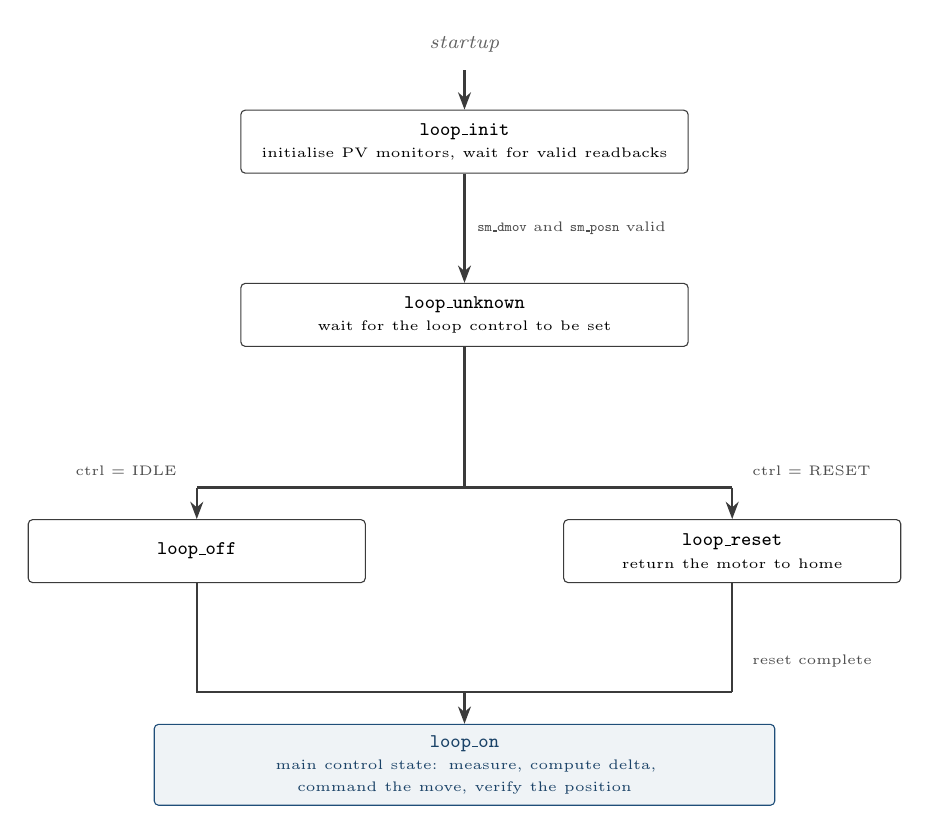
\begin{tikzpicture}[font=\scriptsize, x=1mm, y=1mm]
\def\xC{56}     % centre column

\node[lbl,anchor=south] at (\xC,6) {startup};
\node[blk,text width=54mm,anchor=north] (init) at (\xC,0)
  {\textbf{\texttt{loop\_init}}\\{\tiny initialise PV monitors, wait for valid readbacks}};
\draw[sig] (\xC,5) -- (init.north);

\node[blk,text width=54mm,anchor=north] (unk) at (\xC,-22)
  {\textbf{\texttt{loop\_unknown}}\\{\tiny wait for the loop control to be set}};
\draw[sig] (init.south) -- node[right,tag,xshift=1mm]
  {\texttt{sm\_dmov} and \texttt{sm\_posn} valid} (unk.north);

% the branch: idle or reset
\def\yB{-48}
\draw[draw=cNeut,thick] (unk.south) -- (\xC,\yB);
\draw[draw=cNeut,thick] (22,\yB) -- (90,\yB);
\node[blk,text width=40mm,anchor=north] (off) at (22,\yB-4)
  {\textbf{\texttt{loop\_off}}};
\node[blk,text width=40mm,anchor=north] (rst) at (90,\yB-4)
  {\textbf{\texttt{loop\_reset}}\\{\tiny return the motor to home}};
\draw[sig] (22,\yB) -- (off.north);
\draw[sig] (90,\yB) -- (rst.north);
\node[tag,anchor=south east] at (20,\yB+1) {ctrl $=$ IDLE};
\node[tag,anchor=south west] at (92,\yB+1) {ctrl $=$ RESET};

% both rejoin at loop_on; start the drops at the box edges, not a guessed y
\def\yJ{-74}
\draw[draw=cNeut,thick] (off.south) -- (22,\yJ) -- (90,\yJ);
\draw[draw=cNeut,thick] (rst.south) -- (90,\yJ);
\node[tag,anchor=west] at (92,-70) {reset complete};

\node[ctrl,text width=76mm,anchor=north] (on) at (\xC,\yJ-4)
  {\textbf{\texttt{loop\_on}}\\{\tiny main control state: measure, compute delta,
   command the move, verify the position}};
\draw[sig] (\xC,\yJ) -- (on.north);
\end{tikzpicture}
\end{fitpicture}
\caption{SNL tuner loop state machine. Five states; motion is commanded only from \texttt{loop\_on}.}\label{fig:loop-states}
\end{figure}

\subsection{Guard Checks in loop\_on}\label{sec:guards}


Before the normal control path (\cref{sec:inner-step3}) executes, the \qty{0.5}{\hertz} event handler evaluates guard conditions in priority order:

\begin{longtable}[]{@{}Q{\dimexpr 0.1053\linewidth-1.50\tabcolsep\relax}Q{\dimexpr 0.2895\linewidth-1.50\tabcolsep\relax}Q{\dimexpr 0.3158\linewidth-1.50\tabcolsep\relax}Q{\dimexpr 0.2895\linewidth-1.50\tabcolsep\relax}@{}}
\toprule\noalign{}
Priority & Condition & Status Code & Action \\
\midrule\noalign{}
\endhead
\bottomrule\noalign{}
\endlastfoot
1 & \texttt{loop\_\allowbreak{}ctrl\ =\allowbreak{}=\allowbreak{}\ OFF} & \texttt{LOOP\_\allowbreak{}OFF\_\allowbreak{}STATUS} (1) & No motor action \\
2 & \texttt{meas\_\allowbreak{}count\ =\allowbreak{}=\allowbreak{}\ 0} & \texttt{LOOP\_\allowbreak{}PHASMISS\_\allowbreak{}STATUS} (5) & IQA not producing data \\
3 & Motor stuck \textgreater{} 5 cycles & \texttt{LOOP\_\allowbreak{}SM\_\allowbreak{}MOVE\_\allowbreak{}STATUS} (6) & Motor alarm \\
4 & \texttt{station\_\allowbreak{}state\ =\allowbreak{}=\allowbreak{}\ ON\_\allowbreak{}FM} & \texttt{LOOP\_\allowbreak{}ON\_\allowbreak{}FM\_\allowbreak{}STATUS} (8) & Wait for CW \\
5 & Klystron power low & \texttt{LOOP\_\allowbreak{}LOW\_\allowbreak{}STATUS} (9) & Skip cycle \\
6 & \texttt{dmov\_\allowbreak{}meas\_\allowbreak{}count\ \textless{}\ 1} & --- & Wait for motor idle \\
7 & Motor missed target & \texttt{LOOP\_\allowbreak{}SM\_\allowbreak{}CTRL\_\allowbreak{}STATUS} (7) & Sanity alarm \\
\end{longtable}

Only if all guards pass does the normal path fire (\cref{sec:inner-step3} Step 3).

\subsection{Measurement Accumulator}\label{sec:meas-accum}


A separate \texttt{when(efTest(meas\_\allowbreak{}ready\_\allowbreak{}ef))} block counts measurement events between loop ticks:

\begin{sigblock}
meas_count++
if (sm_dmov == SM_DONE_MOVING):    dmov_meas_count++
else:                               dmov_meas_count = 0
\end{sigblock}

The main control path requires \texttt{dmov\_\allowbreak{}meas\_\allowbreak{}count\ ≥\ LOOP\_\allowbreak{}DMOV\_\allowbreak{}MEAS\ (=\allowbreak{}1)} --- at least one measurement where the motor was idle --- before acting.

\subsection{State Variables and Persistent State}\label{sec:state-vars}


Understanding which variables carry memory across cycles is critical for the upgrade design:

\textbf{Control state (persistent memory --- the loop's "remembrance"):}

\begin{longtable}[]{@{}Q{\dimexpr 0.1769\linewidth-1.33\tabcolsep\relax}Q{\dimexpr 0.2141\linewidth-1.33\tabcolsep\relax}Q{\dimexpr 0.6090\linewidth-1.33\tabcolsep\relax}@{}}
\toprule\noalign{}
Variable & PV & Memory type \\
\midrule\noalign{}
\endhead
\bottomrule\noalign{}
\endlastfoot
\texttt{posn\_ctrl} & \texttt{TUNR:\allowbreak{}POSN:\allowbreak{}CTRL} & \textbf{Inner loop state.} The absolute motor position command. Updated each cycle as \(x_{actual} + \Delta x\). \\
\texttt{LOAD:\allowbreak{}ANGLE:\allowbreak{}UNADOFFS\ .\allowbreak{}VAL} & \texttt{CAV\{N\}LOAD:\allowbreak{}ANGLE:\allowbreak{}UNADOFFS} & \textbf{Outer loop state.} Accumulated strength-error-based corrections with leaky forgetting. Stored in EPICS record \texttt{.VAL}. \\
\end{longtable}

\textbf{Sequencer bookkeeping (SNL-internal):}

\begin{longtable}[]{@{}Q{\dimexpr 0.1739\linewidth-1.00\tabcolsep\relax}Q{\dimexpr 0.8261\linewidth-1.00\tabcolsep\relax}@{}}
\toprule\noalign{}
Variable & Role \\
\midrule\noalign{}
\endhead
\bottomrule\noalign{}
\endlastfoot
\texttt{loop\_state} & Current SNL state (init/off/reset/on) \\
\texttt{loop\_status} & Last computed status code \\
\texttt{prev\_\allowbreak{}loop\_\allowbreak{}ctrl} & Previous cycle's enable value (edge detection + sanity check) \\
\texttt{prev\_\allowbreak{}loop\_\allowbreak{}status} & Last status written to PV (change-detect) \\
\texttt{meas\_count} & Measurement events since the last loop tick \\
\texttt{dmov\_\allowbreak{}meas\_\allowbreak{}count} & Motor-idle measurements (gating condition) \\
\texttt{nomov\_count} & Consecutive stuck-motor cycles \\
\end{longtable}

\textbf{Measured values (stateless --- recomputed each cycle):}

\begin{longtable}[]{@{}Q{\dimexpr 0.4054\linewidth-1.00\tabcolsep\relax}Q{\dimexpr 0.5946\linewidth-1.00\tabcolsep\relax}@{}}
\toprule\noalign{}
Variable & Source \\
\midrule\noalign{}
\endhead
\bottomrule\noalign{}
\endlastfoot
\texttt{posn\_delta} & \texttt{subIQphase2posn} output \\
\texttt{sm\_posn} & Motor record \texttt{.RBV} \\
\texttt{sm\_dmov} & Motor record \texttt{.DMOV} \\
\texttt{station\_state} & \texttt{STN:\allowbreak{}STATE:\allowbreak{}RBCK} \\
\texttt{load\_\allowbreak{}angle\_\allowbreak{}sevr} & \texttt{LOAD:\allowbreak{}ANGLE:\allowbreak{}ERR.\allowbreak{}SEVR} \\
\texttt{klys\_frwd\_pwr} & \texttt{KLYSOUTFRWD:\allowbreak{}POWER} \\
\end{longtable}

\begin{center}\rule{0.5\linewidth}{0.5pt}\end{center}

\section{Disabled Path: Park Mode (PEP-II Only)}\label{sec:park}

\emph{Sources}: \R{4}, \R{11}, \R{14}.


These functions existed for PEP-II (a collider with two rings). In SPEAR3 they are present in the code but permanently disabled. For PEP-II, the nominal park frequency offset was \textbf{±340 kHz} per station: half the cavities were parked at +340 kHz relative to resonance and the other half at −340 kHz \R{15}.

\subsection{Frequency Offset Estimation}\label{sec:park-freq-offset}


\textbf{C function:} \texttt{subSysFreqOff} --- \texttt{rfApp/\allowbreak{}src/\allowbreak{}db/\allowbreak{}subSys.\allowbreak{}c,\allowbreak{}v} line 115 \R{4}\\
\textbf{EPICS record:} \texttt{\$(S):\allowbreak{}\$(C):\allowbreak{}FREQ:\allowbreak{}OFFS}

Estimates frequency offset from tuner position using a polynomial:

\begin{equation}\label{eq:freq-poly}
  f_{offset} = p_0 + p_1 \cdot \Delta x + p_2 \cdot \Delta x^2 + p_3 \cdot \Delta x^3 + t_1 \cdot V_{cav}^2
\end{equation}

where \(\Delta x = \text{Tuner Posn} - \text{ON Home Posn}\) (mm) --- position relative to the ON mode home (\texttt{TUNR:\allowbreak{}POSN:\allowbreak{}ONHOME}), \textbf{not} absolute position. Parameters are calibrated per cavity and thermal conditions. The \(t_1 \cdot V_{cav}^2\) term accounts for RF-heating-induced detuning. The polynomial is typically accurate to \textbf{\textasciitilde10 kHz} per \R{15}.

\textbf{Nominal coefficient ranges} (from \R{15}):

\begin{longtable}[]{@{}Q{\dimexpr 0.3438\linewidth-1.33\tabcolsep\relax}Q{\dimexpr 0.4375\linewidth-1.33\tabcolsep\relax}Q{\dimexpr 0.2188\linewidth-1.33\tabcolsep\relax}@{}}
\toprule\noalign{}
Coefficient & Nominal Range & Units \\
\midrule\noalign{}
\endhead
\bottomrule\noalign{}
\endlastfoot
\(p_0\) & 10 to 20 & kHz \\
\(p_1\) & 20 to 30 & kHz/mm \\
\(p_2\) & 0.4 to 0.6 & kHz/mm² \\
\(p_3\) & −0.01 to +0.01 & kHz/mm³ \\
\(t_1\) & ≈ −0.00010 & kHz/kV² \\
\end{longtable}

\textbf{Output smoothing:} A first-order IIR smoother with \(S = 0.5\) is applied to the frequency offset output before it reaches \texttt{FREQ:ERR} \R{15}:

\begin{equation}\label{eq:freq-smooth}
  f_{smooth}[n] = (1 - S) \cdot f_{offset}[n] + S \cdot f_{smooth}[n-1]
\end{equation}

This halves the effective bandwidth of the polynomial estimate, attenuating noise that could cause excessive motor movement in PARK mode.

\subsection{Park Frequency Error}\label{sec:park-freq-error}


\textbf{C function:} \texttt{subSysFreqErr} --- \texttt{rfApp/\allowbreak{}src/\allowbreak{}db/\allowbreak{}subSys.\allowbreak{}c,\allowbreak{}v} line 147 \R{4}\\
\textbf{EPICS record:} \texttt{\$(S):\allowbreak{}\$(C):\allowbreak{}FREQ:\allowbreak{}ERR}

\begin{equation}\label{eq:freq-err}
  \text{FREQ:ERR} = 0.00004726891 \cdot Q_L \cdot (f_{desired} - f_{offset}) \quad [\text{degrees}]
\end{equation}

This converts a frequency error to phase error in degrees so \texttt{subIQphase2posn} can handle both ON\_CW (phase) and PARK (frequency) paths.

\textbf{Disabled in SPEAR3:} \texttt{INPB} (\(Q_L\) ≈ 7000) is commented out → B=0 → output always 0.

\begin{codeblock}
grecord(sub,"$(S):$(C):FREQ:ERR") {
    field(SNAM,"subSysFreqErr")
    field(INPA,"0.00004726891")   # 90/(476e3 × 4) deg/kHz
  # field(INPB,"7000")            # Q_L — COMMENTED OUT
    field(INPD,"$(S):$(C):FREQ:OFFS.VAL  NPP MS")
}
\end{codeblock}

\begin{center}\rule{0.5\linewidth}{0.5pt}\end{center}

\part{Analysis}

\section{Control Loop Analysis}\label{sec:loop-analysis}


\subsection{Loop Timing Budget}\label{sec:timing-budget}


\Cref{fig:loop-timing} places each contribution to one loop cycle on a common logarithmic time axis. The ratios are what matter: everything in software is negligible against the \qty{2}{\second} period, and the mechanical ramp is the only term of comparable size.

\begin{figure}[tbp]
\centering
\begin{fitpicture}% !TeX root = ../T_tuner_control_analysis.tex
% Tuner loop timing budget on a log time axis.  The point of the figure is the
% ratio, not the individual numbers: software latency is three decades below the
% loop period, and even the mechanical terms sit comfortably inside it.
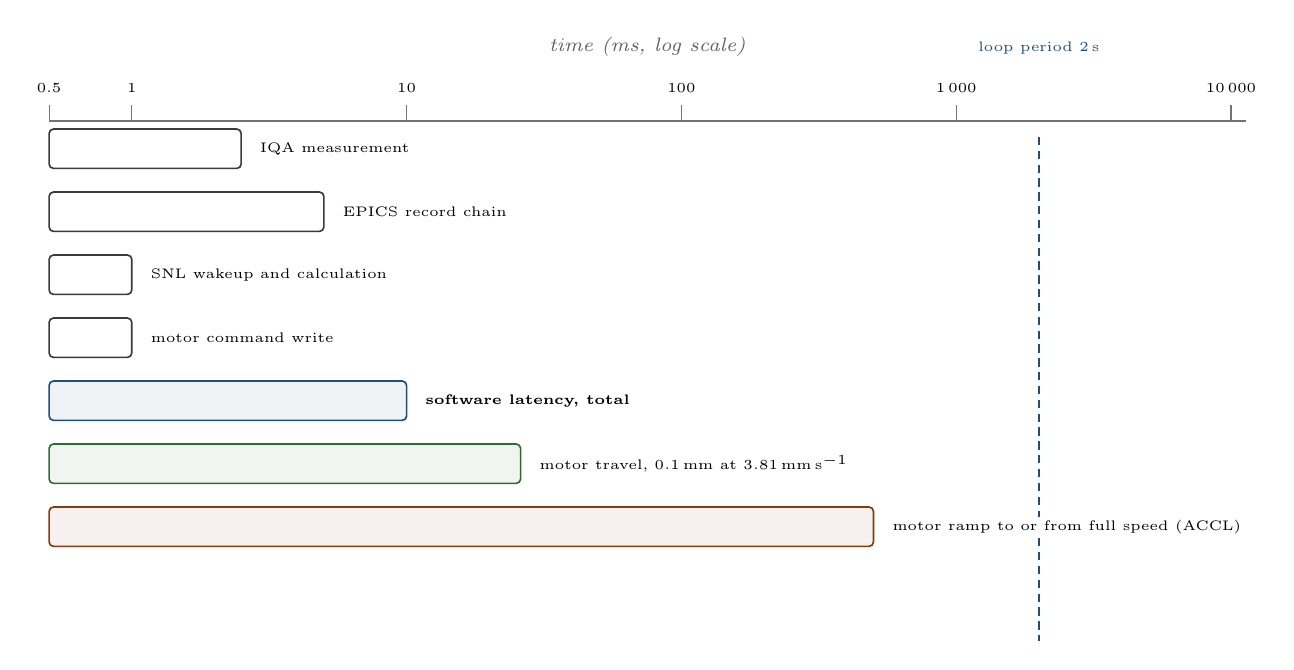
\begin{tikzpicture}[font=\scriptsize, x=1mm, y=1mm]
\pgfmathsetmacro\S{34.9}                       % mm per decade
\newcommand{\px}[1]{(log10(#1)+0.301)*\S}      % t in ms -> x in mm

% ---- axis ----------------------------------------------------------------
\draw[draw=black!55,line width=0.8pt] (0,4) -- (152,4);
\foreach \e/\lab in {-0.301/{0.5}, 0/{1}, 1/{10}, 2/{100}, 3/{1\,000}, 4/{10\,000}}{%
  \pgfmathsetmacro\x{(\e+0.301)*\S}
  \draw[draw=black!55] (\x,4) -- (\x,6);
  \node[font=\tiny,anchor=south] at (\x,6.4) {\lab};
}
\node[lbl,anchor=south] at (76,11) {time (ms, log scale)};

% ---- the 2 s loop period, as the reference the rest is judged against ----
\pgfmathsetmacro\xp{\px{2000}}
\draw[draw=cCtrl,line width=1pt,densely dashed] (\xp,2) -- (\xp,-62);
\node[tag,text=cCtrl,anchor=south] at (\xp,12)
  {loop period \qty{2}{\second}};

% ---- budget bars ---------------------------------------------------------
% {label}/{t in ms}/{row}/{style}
\foreach \lab/\t/\r/\sty in {%
  {IQA measurement}/2.5/0/blk,
  {EPICS record chain}/5/1/blk,
  {SNL wakeup and calculation}/1/2/blk,
  {motor command write}/1/3/blk,
  {\bfseries software latency, total}/10/4/ctrl,
  {motor travel, \qty{0.1}{\milli\metre} at \qty{3.81}{\milli\metre\per\second}}/26/5/rf,
  {motor ramp to or from full speed (ACCL)}/500/6/pwr}{%
    \pgfmathsetmacro\y{-2-\r*8}
    \pgfmathsetmacro\x{\px{\t}}
    \draw[\sty,fill,draw,line width=0.6pt] (0,\y) rectangle (\x,\y+5);
    % fill=white so a label that runs past the loop-period marker masks it
    \node[font=\tiny,anchor=west,fill=white,inner sep=1pt] at (\x+2,\y+2.5) {\lab};
}
\end{tikzpicture}
\end{fitpicture}
\caption[Tuner loop timing budget.]{Timing of one tuner loop cycle. Every contribution, mechanical ones included, sits inside the \qty{2}{\second} loop period; the software terms are three decades below it.}\label{fig:loop-timing}
\end{figure}

\subsection{Open-Loop Gain (Proportional Path)}\label{sec:open-loop-gain}


The linearized loop gain from phase error to stepper position change per cycle:

\begin{equation}\label{eq:gol}
  G_{OL} = C_{mm/deg} \cdot G_{loop} = 0.020\text{–0.030} \; \frac{\text{mm}}{\text{°}} \cdot G_{loop}
\end{equation}

A position change of \(\Delta x\) mm changes cavity resonant frequency by:

\begin{equation}\label{eq:dfdx}
  \frac{df}{dx} \approx p_1 \quad [\text{kHz/mm}]
\end{equation}

(the linear coefficient of the tuner polynomial, calibrated per cavity)

\textbf{Effective loop gain} (phase domain, per cycle with \(G_{loop}=1\)):

\begin{equation}\label{eq:geff}
  G_{eff} = C_{mm/deg} \cdot p_1 \cdot \frac{90°}{4 f_0} \cdot Q_L
\end{equation}

For nominal values (\(C = 0.020\) mm/° (lower end of range), \(p_1 \approx 10\) kHz/mm, \(Q_L \approx 7000\), \(f_0 = 476\) MHz):

\begin{equation}\label{eq:geff-num}
  G_{eff} \approx 0.02 \times 10 \times 0.00004726891 \times 10^3 \times 7000 \approx 66
\end{equation}

\begin{keynote}
\textbf{Note:} \Cref{eq:geff-num} is the single-cycle proportional gain. The \qty{0.5}{\hertz} rate and motor velocity limit prevent instability by severely band-limiting the loop. \texttt{CAVTUNR:\allowbreak{}LOOP:\allowbreak{}GAIN} (0--1) is critical for stability.

The factor \(90°/4f_0\) in \cref{eq:geff} is the constant \texttt{0.00004726891} that \texttt{subSysFreqErr} uses \R{4}. That routine documents it as the \emph{park} frequency-error scaling (degrees per kHz per unit \(Q_L\)), which is about five times smaller than the physical load-angle conversion in \cref{eq:theta-to-df}. Whether the inner-loop gain estimate should use the park constant or the physical one has not been resolved here; the qualitative conclusion --- \(G_{eff} \gg 1\), so the loop gain scalar is what keeps the loop stable --- holds either way.\openitem{O8}
\end{keynote}

\subsection{Integrator Dynamics (Outer Loop)}\label{sec:integrator-dynamics}


The load angle offset integrator is a \textbf{leaky first-order IIR integrator},
\cref{eq:integrator}. Its two tuning constants set the DC gain and the leak rate.

\textbf{K gain} (\texttt{CAVLOAD:\allowbreak{}ANGLE:\allowbreak{}K}, deg/\%): Per-sample step size. \texttt{DRVH=1} limits K ≤ 1 deg/\%.

\textbf{Forgetting factor} (\texttt{CAVLOAD:\allowbreak{}ANGLE:\allowbreak{}FORGET}, 0 \textless{} forget ≤ 1): Makes the integrator leaky:

\begin{itemize}
\tightlist
\item
  \textbf{DC gain:} \(G_{DC} = -K/(1 - \text{forget})\) deg/\%
\item
  \textbf{Decay time constant:} \(\tau = -T / \ln(\text{forget})\) where \(T = \qty{2}{\second}\) is the loop period
\item
  If the strength error disappears, the accumulated offset decays to zero with time constant \(\tau\)
\end{itemize}

\begin{longtable}[]{@{}Q{\dimexpr 0.0857\linewidth-1.50\tabcolsep\relax}Q{\dimexpr 0.2714\linewidth-1.50\tabcolsep\relax}Q{\dimexpr 0.2714\linewidth-1.50\tabcolsep\relax}Q{\dimexpr 0.3714\linewidth-1.50\tabcolsep\relax}@{}}
\toprule\noalign{}
\texttt{forget} & \(\tau\) (seconds) & DC gain (K=1 deg/\%) & Notes \\
\midrule\noalign{}
\endhead
\bottomrule\noalign{}
\endlastfoot
1.000 & ∞ (pure integrator) & ∞ & Winds up indefinitely \\
0.999 & ≈ 2000 s (33 min) & −1000 deg/\% & Very slow, high-gain \\
0.990 & ≈ 200 s (3.3 min) & −100 deg/\% & Moderate --- typical range \\
0.900 & ≈ 19 s & −10 deg/\% & Aggressive \\
\end{longtable}

\begin{keynote}
\textbf{Configuration note:} Both K and FORGET are \texttt{ao} records with \texttt{PINI=YES} but no hardcoded defaults. On a fresh start without autosave, both = 0, silently disabling the integrator.
\end{keynote}

\subsection{Bandwidth Hierarchy and Disturbance Rejection}\label{sec:bandwidth}


\begin{itemize}
\tightlist
\item
  Inner proportional loop bandwidth: \textasciitilde0.01--0.05 Hz (operator-tunable via \texttt{LOOP:GAIN})
\item
  Outer integrator loop bandwidth: \textasciitilde0.0001--0.008 Hz (set by K and forget; \(f \approx 1/2\pi\tau\))
\end{itemize}

\textbf{Primary disturbance --- beam loading:} The dominant source of cavity detuning. As beam is injected, decays, or is lost, \(\Delta f \propto I_{b1} \sin\phi_s / V_{gap}\) (\cref{eq:detune-beam}) shifts the cavity resonance. Under normal SPEAR3 operation (slow current decay, hours lifetime), the average detuning rate is slow enough for the \qty{0.5}{\hertz} loop. However, discrete events --- injection bursts, fast beam loss --- can shift detuning faster than the \qty{2}{\second} loop period.

\textbf{Secondary disturbance --- thermal drift:} RF heating shifts resonant frequency on minutes-to-hours timescale. Much smaller than beam loading at SPEAR3 gradients. Easily handled by the inner loop.

\textbf{Uncorrected disturbances:} Fast detuning transients (injection events, beam loss) and components \textgreater{} \textasciitilde0.25 Hz are not corrected by the \qty{0.5}{\hertz} loop. These manifest as transient phase errors that ring down over several loop cycles.

\begin{center}\rule{0.5\linewidth}{0.5pt}\end{center}

\section{Hardware Interface}\label{sec:hardware}

\emph{Sources}: \R{6}, \R{7}, \R{8}, \R{12}, \R{16}.


\subsection{Stepper Motor Record}\label{sec:motor-record}


\textbf{EPICS record type:} \texttt{steppermotor} (custom AB 1746-HSTP1 driver record)\\
\textbf{Physical device (legacy):} Allen-Bradley 1746-HSTP1 stepper module\\
\textbf{Physical device (in development, not installed):} Galil DMC-4143 motion controller\openitem{O7}

\begin{codeblock}
grecord(steppermotor,"$(S):$(C)TUNR:STEP:MOTOR") {
    field(DTYP,"AB-1746HSTP1")
    field(OUT,"#L0 A2 C$(M) S0 @@0x8413 0x0010 500")
    field(DOL,"$(S):$(C)TUNR:POSN:CTRL.VAL  NPP NMS")
    field(OMSL,"closed_loop")
    field(ACCL,".5")          # seconds to reach velocity
    field(VELO,"3")           # velocity: 3 rev/s = 3.81 mm/s
    field(DIST,"0.003175")    # mm per step
    field(MODE,"Position")
    field(CMOD,"Position")
    field(MRES,"400")         # steps per revolution
    field(PREC,"3")
    field(EGU,"mm")
    field(DRVH,"18")          # upper drive limit: +18 mm
    field(DRVL,"-29.5")       # lower drive limit: -29.5 mm
    field(RDBD,"0.015875")    # retry deadband: 5 steps
}
\end{codeblock}

\subsection{Mechanism Specifications}\label{sec:mechanism}


\begin{longtable}[]{@{}Q{\dimexpr 0.3944\linewidth-1.33\tabcolsep\relax}Q{\dimexpr 0.2254\linewidth-1.33\tabcolsep\relax}Q{\dimexpr 0.3803\linewidth-1.33\tabcolsep\relax}@{}}
\toprule\noalign{}
Parameter & Value & Calculation \\
\midrule\noalign{}
\endhead
\bottomrule\noalign{}
\endlastfoot
Step resolution & 0.003175 mm/step & 1.27 mm/rev ÷ 400 steps/rev \\
Retry deadband & 0.015875 mm & 5 steps exactly \\
Maximum velocity & 3.81 mm/s & VELO 3 rev/s × MRES 400 steps/rev × DIST 0.003175 mm/step \\
Acceleration & 7.62 mm/s² & ACCL = 0.5 s to reach full velocity \\
Travel range & 47.5 mm total & −29.5 to +18 mm \\
Time to traverse full range & \textasciitilde12.5 s & 47.5 mm at 3.81 mm/s \\
Time to stop from full speed & 0.5 s & ACCL is specified directly as seconds to velocity \\
Min detectable move & 0.015875 mm & 1 RDBD = 5 steps \\
\end{longtable}

These are the \emph{commanded} limits taken from the motor record \R{8}. They
assume the mechanism itself is free over the whole range: the June 2023 tuner
inspection recorded bellows and mechanical-stop problems on cavities A and B and
a limit-switch problem on cavity C, and whether those were repaired is not
recorded here.\openitem{O6}

\subsection{Position Control and Initialization}\label{sec:position-init}


The motor uses \textbf{absolute position mode}. On IOC startup:

\begin{enumerate}
\def\labelenumi{\arabic{enumi}.}
\tightlist
\item
  \texttt{TUNR:\allowbreak{}STEP:\allowbreak{}CHCKINIT} verifies motor is initialized
\item
  \texttt{TUNR:\allowbreak{}STEP:\allowbreak{}INIT} sequence captures current hardware position → \texttt{TUNR:\allowbreak{}POSN:\allowbreak{}CTRL}
\item
  Subsequent commands write to \texttt{TUNR:\allowbreak{}POSN:\allowbreak{}CTRL}, which FLNKs directly to the motor record
\end{enumerate}

\begin{center}\rule{0.5\linewidth}{0.5pt}\end{center}

\section{Design Gaps and Upgrade Opportunities}\label{sec:gaps}

\emph{Sources}: \R{8}, \R{15}, \R{17}.


\subsection{Commented-Out Parameters Make Tuner Non-Functional on Fresh Start}\label{sec:gap-commented}


The three key parameters for \texttt{subIQphase2posn} (deadband B, conversion C, max-delta D) are commented out in the database. On a clean start without autosave restore, C=0 → no motor movement, D=0 → output clamped to 0.

\textbf{Recommendation:} Encode these as \texttt{ao} records with \texttt{PINI=YES} and default values.

\subsection{Outer Loop Disabled on Fresh Start (Functional with Autosave)}\label{sec:gap-outer-disabled}


The LOAD:ANGLE:OFFS bounds (INPC) are commented out in the DB source (\texttt{\#field(INPC,\allowbreak{}"10")}): \texttt{clamp(val,\allowbreak{}\ 0,\allowbreak{}\ 0)\ =\allowbreak{}\ 0} on a fresh IOC start without autosave. In normal operation with autosave restore, INPC is restored to 75° \R{15}, making the outer loop potentially active when \texttt{LOAD:\allowbreak{}ANGLE:\allowbreak{}CTRL=\allowbreak{}1}. Additionally, K and FORGET have no hardcoded DB defaults (both = 0 on fresh start without autosave).

\textbf{Risk:} On a fresh IOC start without autosave (disaster recovery, new deployment), the outer loop is silently non-functional. An operator setting \texttt{LOAD:\allowbreak{}ANGLE:\allowbreak{}CTRL=\allowbreak{}1} may believe the outer loop is active when it is not.

\textbf{Recommendation:} Encode explicit defaults for K (0.5 deg/\%), FORGET (0.9995), and OFFS bounds (±75°) as DB \texttt{PINI=YES} values in the upgrade design.

\subsection{No Feedforward for Beam Loading}\label{sec:gap-feedforward}


Beam loading is the primary disturbance (\cref{sec:why-tuner}, \cref{sec:bandwidth}). The only compensation path is the \qty{0.5}{\hertz} reactive inner loop. The outer integrator was designed to find optimal detuning implicitly, but is inactive. Even if active, its \textasciitilde50 s time constant cannot respond to injection transients.

\textbf{There is no feedforward from beam current to detuning setpoint.} This leaves the cavity transiently detuned during injection and loss events.

\textbf{Upgrade opportunity:} Real-time detuning feedforward from DCCT beam current, using \cref{eq:detune-beam} directly:

\begin{equation}\label{eq:feedforward}
  \Delta f_{ff} = -\frac{f_0}{2}\cdot\frac{R}{Q}\cdot\frac{I_{b1}\sin\phi_s}{V_{gap}}
\end{equation}

Computable in the LLRF9 with sub-millisecond latency.

\subsection{Implicit vs. Explicit Physics}\label{sec:gap-implicit}


The legacy system uses an implicit integrator to find optimal detuning rather than first-principles computation (\(\psi_{opt} = \arctan(2Q_L \Delta\omega / \omega_0)\)). This is robust but slow.

\textbf{Upgrade opportunity:} Explicit model-based \(\Delta f_{opt}\) from measured \(I_b\), \(V_{gap}\), and \(\phi_s\) --- directly enabled by LLRF9 DSP.

\subsection{Motor Resolution vs. Phase Resolution}\label{sec:gap-resolution}


With C = 0.020 mm/° (minimum end of nominal range; worst-case resolution):

\begin{itemize}
\tightlist
\item
  1 step (0.003175 mm) ≡ 0.159° phase change
\item
  RDBD (5 steps = 0.015875 mm) ≡ 0.794° phase
\end{itemize}

For \(Q_L \approx 7000\): 0.159° corresponds to \(\Delta f \approx 95\) Hz minimum resolvable correction. The Galil controller would achieve sub-step positioning once commissioned.

\subsection{No State Estimation or Predictive Control}\label{sec:gap-estimation}


Purely reactive --- responds to measured error with no prediction. The \qty{0.5}{\hertz} rate cannot correct disturbances above its \qty{0.25}{\hertz} Nyquist limit (AC ripple, beam chopping).

\subsection{Outer Loop Trigger Is SNL-Mediated}\label{sec:gap-trigger}


The outer integrator is triggered by the SNL writing PROC, not by the scan record. If the sequencer is not running (IOC restart, task crash) or the motor is persistently stuck (\texttt{DMOV=0}), the outer loop freezes silently.

\textbf{Recommendation:} Consider independent scan-based outer loop in upgrade.

\subsection{Voltage Loop Sign Ambiguity --- Lorentzian Symmetry Problem}\label{sec:gap-sign}


\textbf{This is a fundamental control-design vulnerability in the outer (voltage) loop.}

The cavity voltage response vs. detuning is a Lorentzian:

\begin{equation}\label{eq:lorentzian}
  V(\Delta f) = \frac{V_{max}}{\sqrt{1 + \left(\frac{2 Q_L \,\Delta f}{f_0}\right)^2}}
\end{equation}

This curve is \textbf{symmetric around resonance} --- the same reduced voltage appears at \(+\Delta f\) and \(-\Delta f\). The integrator uses voltage error alone (\texttt{STRENGTH\ −\ STRENGTH:\allowbreak{}CTRL}) to decide which direction to push the phase offset:

\begin{codeblock}
psub->val -= psub->l * psub->j;   // offset -= (actual − desired) × K
\end{codeblock}

When voltage is too low (actual \textless{} desired), the integrator always \textbf{increases} the offset. This is correct only if the cavity is detuned on one side of resonance. If it happens to be on the other side:

\begin{sigblock}
Scenario: cavity detuned ABOVE resonance (Δf > 0)
  → voltage < target  (down the Lorentzian slope)
  → error = actual − desired < 0
  → offset -= (negative × K) → offset INCREASES
  → inner loop drives tuner further above resonance
  → voltage drops MORE → error grows → offset increases faster
  → POSITIVE FEEDBACK → runaway to ±180° clamp
\end{sigblock}

The integrator converges only from the \textbf{correct side} of resonance; from the wrong side it diverges. Which side is "correct" depends on the sign of K and the tuner geometry (sign of \(df/dx\)), but the fundamental issue is that voltage alone does not distinguish \(+\Delta f\) from \(-\Delta f\).

\textbf{Why this doesn't cause problems in practice:} In SPEAR3 as deployed, the outer loop is non-functional on fresh start (see \cref{sec:outer-total}, \cref{sec:gap-outer-disabled}). The inner loop uses phase error, which is \textbf{monotonic} with detuning (not symmetric), so it does not have this ambiguity. If the outer loop were ever activated (e.g., via autosave with Max Offs = 75°):

\begin{enumerate}
\def\labelenumi{\arabic{enumi}.}
\tightlist
\item
  \textbf{Normal operation (beam loading dominant):} Beam loading consistently pulls the cavity to one side of resonance (determined by \(\sin\phi_s\)). If the initial sign convention is chosen for this side, convergence is reliable under steady-state conditions.
\item
  \textbf{Transient risk:} After a beam loss/injection event, the cavity could briefly end up on the wrong side of resonance. The integrator would push in the wrong direction until either (a) the inner loop's phase control pulls it back, or (b) the offset hits the ±180° clamp.
\item
  \textbf{Startup ambiguity:} On first activation, the cavity's initial detuning direction is unknown. The integrator has a 50/50 chance of guessing wrong.
\end{enumerate}

\textbf{Upgrade recommendation:} Any replacement for the voltage loop should use \textbf{signed detuning information} (available from the phase measurement) rather than unsigned voltage error. Options include:

\begin{itemize}
\tightlist
\item
  Feedforward from beam current (\cref{sec:gap-feedforward}) --- eliminates the need for voltage feedback entirely
\item
  Model-based optimal detuning (\cref{sec:gap-implicit}) --- computes \(\Delta f_{opt}\) directly from \(I_b\), \(V_{gap}\), \(\phi_s\)
\item
  If a voltage feedback loop is retained, include sign discrimination by checking the inner loop's phase error sign to determine which side of resonance the cavity is on, and flip the integrator sign accordingly
\end{itemize}

\begin{center}\rule{0.5\linewidth}{0.5pt}\end{center}

\section{Operational Summary: SPEAR3 As Deployed}\label{sec:operational}


\textbf{In SPEAR3 as deployed, the tuner operates exclusively in pure resonance-seeking mode:}

\begin{enumerate}
\def\labelenumi{\arabic{enumi}.}
\item
  \textbf{Inner loop (active):} \qty{0.5}{\hertz} proportional phase controller. Error = \texttt{PROBE:\allowbreak{}PHASE.\allowbreak{}L\ −\ FRWD:\allowbreak{}PHASE.\allowbreak{}L}. Motor drives to nullify this error → cavity stays at the calibrated resonant frequency.
\item
  \textbf{Outer loop (inactive on fresh start; potentially active with autosave):} The \texttt{LOAD:\allowbreak{}ANGLE:\allowbreak{}OFFS} max bound (INPC) is commented out in the DB source --- on a fresh start \texttt{clamp(val,\allowbreak{}\ 0,\allowbreak{}\ 0)\ =\allowbreak{}\ 0} discards the integrator output. In normal SPEAR3 operation, autosave restores INPC to 75°, allowing the outer loop to function when \texttt{LOAD:\allowbreak{}ANGLE:\allowbreak{}CTRL=\allowbreak{}1}. In practice at SPEAR3 with modest beam loading the outer loop has always run at \(\theta_{offset} = 0\) (pure resonance-seeking mode). See \cref{sec:outer-total} and \cref{sec:gap-outer-disabled}.
\item
  \textbf{PARK mode (disabled):} Permanently disabled via commented-out \texttt{INPB} in \texttt{FREQ:ERR}.
\end{enumerate}

\textbf{What "resonance" means here:} The calibrated zero reference from the no-beam IQA calibration procedure (\cref{sec:iqa-calibration}). The system keeps \texttt{probe\_\allowbreak{}phase\ −\ fwd\_\allowbreak{}phase\ =\allowbreak{}\ 0}, which equals resonance only if the calibration is valid.

\textbf{What is NOT compensated:} With \(\theta_{offset} = 0\), the tuner always drives toward zero detuning (resonance). It does not apply the optimal detuning angle that would minimize generator power under beam loading. For SPEAR3's modest beam loading this is acceptable. For higher beam loading conditions, the outer voltage loop exists in the architecture but requires explicit configuration to activate.

\begin{center}\rule{0.5\linewidth}{0.5pt}\end{center}

\appendix

\appendix

\section{Complete EPICS Signal Chain}\label{app:signal-chain}


\subsection{Data Flow (SPEAR3 ON\_CW Mode)}\label{app:data-flow}


\begin{sigblock}
Step 1: IQA hardware acquires I,Q at 400 Hz
  SRF1:CAV1PROBE:IQ → subIQphase → SRF1:CAV1PROBE:PHASE  (degrees, unadjusted in .L)
  SRF1:CAV1FRWD:IQ  → subIQphase → SRF1:CAV1FRWD:PHASE   (degrees, unadjusted in .L)

Step 2: Load angle target (slow integrator, if enabled)
  SRF1:CAV1:STRENGTH (= probe_amplitude / station_voltage × 100%)
  SRF1:CAV1:STRENGTH:CTRL (operator setpoint, %)
  → SRF1:CAV1LOAD:ANGLE:UNADOFFS (subIQphaseOffsU, triggered by SNL)
  → SRF1:CAV1LOAD:ANGLE:OFFS     (subIQphaseOffs, = fixed_offs + unadj_offs, bounded)

Step 3: Load angle error
  SRF1:CAV1LOAD:ANGLE:ERR (subIQphaseErr):
    error = PROBE:PHASE.L − FRWD:PHASE.L + LOAD:ANGLE:OFFS
    wrapped to [−180°, +180°]

Step 4: Phase error to position delta
  SRF1:CAV1TUNR:POSN:DELTA (subIQphase2posn):
    if |error| > deadband_B:
        delta = error × C_mm_per_deg × gain_E
        delta = clamp(delta, −D_mm, +D_mm)
    else:
        delta = 0
  → fires event SRF1:CAVTUNR:LOOP:READY

Step 5: SNL sequencer (one instance per cavity)
  Wakes on READY event
  new_posn = sm_posn + posn_delta
  new_posn = clamp(new_posn, sm_drvl, sm_drvh)
  writes new_posn → SRF1:CAV1TUNR:POSN:CTRL

Step 6: Motor response
  SRF1:CAV1TUNR:POSN:CTRL FLNK → SRF1:CAV1TUNR:STEP:MOTOR
  Motor moves to absolute position new_posn
  Readback: SRF1:CAV1TUNR:POSN (motor .RBV → EPICS ao)
\end{sigblock}

\subsection{Record Trigger Chain}\label{app:trigger-chain}


\begin{sigblock}
SRF1:CAVTUNR:LOOP:SEQ  [SCAN="2 second"]
    → fires FLNK → SRF1:CAVTUNR:LOOP:READY (event)
    → SRF1:CAV{1,2,3,4}TUNR:POSN:DELTA processes (event-triggered)
        → each POSN:DELTA FLNK → SRF1:CAV{N}TUNR:LOOPMEAS:READY event
            → wakes SNL sequencer instance (per cavity)
                → SNL reads posn_delta, updates motor: pvPut(TUNR:POSN:CTRL)
                → SNL writes PROC to LOAD:ANGLE:UNADOFFS (via phase_offset_proc)
                    → subIQphaseOffsU fires → updates voltage integrator
                    → FLNK → LOAD:ANGLE:OFFS recomputed
                        → feeds next cycle's LOAD:ANGLE:ERR
\end{sigblock}

\begin{center}\rule{0.5\linewidth}{0.5pt}\end{center}

\section{Parameter Reference}\label{app:parameters}


\subsection{Operator-Settable Parameters (Station-Level)}\label{app:param-station}


These are \texttt{ao}/\texttt{bo} records in \texttt{rf\_\allowbreak{}stn\_\allowbreak{}cav.\allowbreak{}db,\allowbreak{}v}, shared across all cavities (prefix \texttt{\$(S):CAV}):

\begin{longtable}[]{@{}Q{\dimexpr 0.3049\linewidth-1.67\tabcolsep\relax}Q{\dimexpr 0.0488\linewidth-1.67\tabcolsep\relax}Q{\dimexpr 0.0610\linewidth-1.67\tabcolsep\relax}Q{\dimexpr 0.0488\linewidth-1.67\tabcolsep\relax}Q{\dimexpr 0.0976\linewidth-1.67\tabcolsep\relax}Q{\dimexpr 0.4390\linewidth-1.67\tabcolsep\relax}@{}}
\toprule\noalign{}
PV (with prefix \texttt{SRF1:CAV}) & Type & EGU & DRVH & Default & Description \\
\midrule\noalign{}
\endhead
\bottomrule\noalign{}
\endlastfoot
\texttt{TUNR:\allowbreak{}LOOP:\allowbreak{}CTRL} & bo & --- & --- & --- & Master loop enable (0=off, 1=on) \\
\texttt{TUNR:\allowbreak{}LOOP:\allowbreak{}GAIN} & ao & --- & 1 & autosave & Phase-to-position gain scalar (0--1) \\
\texttt{LOAD:ANGLE:K} & ao & deg/\% & 1 & autosave & Integrator K constant \\
\texttt{LOAD:\allowbreak{}ANGLE:\allowbreak{}FORGET} & ao & --- & 1 & autosave & Forgetting factor (≤1) \\
\texttt{LOAD:\allowbreak{}ANGLE:\allowbreak{}ERRMAX} & ao & deg & 180 & autosave & Max allowed load angle error \\
\texttt{LOAD:\allowbreak{}ANGLE:\allowbreak{}CTRL} & bo & --- & --- & autosave & Enable load angle offset integrator \\
\texttt{STRENGTH:CTRL} & ao & \% & 100 & autosave & Desired cavity strength setpoint (\%) \\
\texttt{STRENGTH:DIFF} & ao & \% & 100 & autosave & Voltage integrator deadband \\
\end{longtable}

\subsection{Per-Cavity Parameters (rf\_cav.db,v)}\label{app:param-cavity}


\begin{longtable}[]{@{}Q{\dimexpr 0.2247\linewidth-1.50\tabcolsep\relax}Q{\dimexpr 0.3820\linewidth-1.50\tabcolsep\relax}Q{\dimexpr 0.0899\linewidth-1.50\tabcolsep\relax}Q{\dimexpr 0.3034\linewidth-1.50\tabcolsep\relax}@{}}
\toprule\noalign{}
PV (e.g., \texttt{SRF1:CAV1}) & Function & Default & Notes \\
\midrule\noalign{}
\endhead
\bottomrule\noalign{}
\endlastfoot
\texttt{TUNR:\allowbreak{}POSN:\allowbreak{}ONHOME} & Home position for freq polynomial & autosave & Reference for \texttt{subSysFreqOff} \\
\texttt{TUNR:\allowbreak{}POSN:\allowbreak{}PARKHOME} & Park home position & autosave & PEP-II only \\
\texttt{LOAD:\allowbreak{}ANGLE:\allowbreak{}OFFS} & Total load angle offset (computed) & 0 & output of \texttt{subIQphaseOffs} \\
\end{longtable}

\subsection{Commented-Out Parameters (Require Autosave)}\label{app:param-commented}


\begin{longtable}[]{@{}Q{\dimexpr 0.1403\linewidth-1.60\tabcolsep\relax}Q{\dimexpr 0.0468\linewidth-1.60\tabcolsep\relax}Q{\dimexpr 0.1424\linewidth-1.60\tabcolsep\relax}Q{\dimexpr 0.2314\linewidth-1.60\tabcolsep\relax}Q{\dimexpr 0.4391\linewidth-1.60\tabcolsep\relax}@{}}
\toprule\noalign{}
Sub Record & Input & Function & Design Value & Status \\
\midrule\noalign{}
\endhead
\bottomrule\noalign{}
\endlastfoot
\texttt{TUNR:\allowbreak{}POSN:\allowbreak{}DELTA} & INPB & Phase deadband (°) & 0.25 & \texttt{\#field(INPB,\allowbreak{}"0.\allowbreak{}25")} --- commented \\
\texttt{TUNR:\allowbreak{}POSN:\allowbreak{}DELTA} & INPC & mm per degree & 0.020--0.030 range & \texttt{\#field(INPC,\allowbreak{}"0.\allowbreak{}02")} --- commented \\
\texttt{TUNR:\allowbreak{}POSN:\allowbreak{}DELTA} & INPD & Max delta per cycle (mm) & 1.0 & \texttt{\#field(INPD,\allowbreak{}"1")} --- commented \\
\texttt{LOAD:\allowbreak{}ANGLE:\allowbreak{}OFFS} & INPC & Max offset bound (°) & 10 (DB); \textbf{75 operational} \R{15} & \texttt{\#field(INPC,\allowbreak{}"10")} --- commented; autosave restores 75° in normal operation \\
\texttt{FREQ:ERR} & INPB & Loaded cavity Q & 7000 & \texttt{\#field(INPB,\allowbreak{}"7000")} --- commented \\
\end{longtable}

\subsection{Physical Constants (Hardwired)}\label{app:param-constants}


\begin{longtable}[]{@{}Q{\dimexpr 0.1648\linewidth-1.50\tabcolsep\relax}Q{\dimexpr 0.2308\linewidth-1.50\tabcolsep\relax}Q{\dimexpr 0.2857\linewidth-1.50\tabcolsep\relax}Q{\dimexpr 0.3187\linewidth-1.50\tabcolsep\relax}@{}}
\toprule\noalign{}
Constant & Value & Location & Meaning \\
\midrule\noalign{}
\endhead
\bottomrule\noalign{}
\endlastfoot
\texttt{90/\allowbreak{}(476e3\ ×\ 4)} & 0.00004726891 deg/kHz & \texttt{rf\_cav.db,v}, FREQ:ERR INPA & Phase per unit frequency \\
RF frequency & 476 MHz & Implicit & SPEAR3 accelerating frequency \\
Stepper DIST & 0.003175 mm/step & Motor record & Linear resolution \\
Stepper MRES & 400 steps/rev & Motor record & Angular resolution \\
Stepper RDBD & 0.015875 mm & Motor record & 5-step retry deadband \\
Motor DRVH/DRVL & +18 / −29.5 mm & Motor record & Travel limits \\
Motor VELO & 3 rev/s (= 3.81 mm/s) & Motor record & Maximum velocity \\
Motor ACCL & 0.5 s & Motor record & Seconds to reach velocity (= 7.62 mm/s²) \\
\end{longtable}

\begin{center}\rule{0.5\linewidth}{0.5pt}\end{center}

\section{SNL Variables, Constants, and Status Codes}\label{app:snl}


\subsection{Complete PV Binding Table}\label{app:snl-pv}


\begin{longtable}[]{@{}Q{\dimexpr 0.2128\linewidth-1.50\tabcolsep\relax}Q{\dimexpr 0.0638\linewidth-1.50\tabcolsep\relax}Q{\dimexpr 0.3617\linewidth-1.50\tabcolsep\relax}Q{\dimexpr 0.3617\linewidth-1.50\tabcolsep\relax}@{}}
\toprule\noalign{}
SNL Variable & Type & EPICS PV & Role \\
\midrule\noalign{}
\endhead
\bottomrule\noalign{}
\endlastfoot
\texttt{loop\_ctrl} & int & \texttt{\{STN\}:\allowbreak{}CAVTUNR:\allowbreak{}LOOP:\allowbreak{}CTRL} & Master enable, monitored (bo) \\
\texttt{loop\_state} & int & \texttt{\{STN\}:\allowbreak{}CAV\{CAV\}TUNR:\allowbreak{}LOOP:\allowbreak{}STATE} & Output: current SNL state code \\
\texttt{loop\_status} & int & \texttt{\{STN\}:\allowbreak{}CAV\{CAV\}TUNR:\allowbreak{}LOOP:\allowbreak{}STATUS} & Output: status code \\
\texttt{loop\_\allowbreak{}status\_\allowbreak{}string\_\allowbreak{}c} & string & \texttt{\{STN\}:\allowbreak{}CAV\{CAV\}TUNR:\allowbreak{}LOOP:\allowbreak{}STRING} & Output: human-readable status text \\
\texttt{station\_state} & int & \texttt{\{STN\}:\allowbreak{}STN:\allowbreak{}STATE:\allowbreak{}RBCK} & Monitored, drives state branching \\
\texttt{posn\_ctrl} & float & \texttt{\{STN\}:\allowbreak{}CAV\{CAV\}TUNR:\allowbreak{}POSN:\allowbreak{}CTRL} & Motor position command (mm) \\
\texttt{posn\_delta} & float & \texttt{\{STN\}:\allowbreak{}CAV\{CAV\}TUNR:\allowbreak{}POSN:\allowbreak{}DELTA} & Per-cycle position increment \\
\texttt{posn\_new} & float & \texttt{\{STN\}:\allowbreak{}CAV\{CAV\}TUNR:\allowbreak{}POSN:\allowbreak{}LOOP} & Logged: newly computed target \\
\texttt{posn} & float & \texttt{\{STN\}:\allowbreak{}CAV\{CAV\}TUNR:\allowbreak{}POSN} & Potentiometer position readback \\
\texttt{posn\_on\_home} & float & \texttt{\{STN\}:\allowbreak{}CAV\{CAV\}TUNR:\allowbreak{}POSN:\allowbreak{}ONHOME} & Home for ON mode \\
\texttt{posn\_\allowbreak{}park\_\allowbreak{}home} & float & \texttt{\{STN\}:\allowbreak{}CAV\{CAV\}TUNR:\allowbreak{}POSN:\allowbreak{}PARKHOME} & Home for PARK (PEP-II) \\
\texttt{posn\_mdel} & float & \texttt{\{STN\}:\allowbreak{}CAV\{CAV\}TUNR:\allowbreak{}POSN.\allowbreak{}MDEL} & Monitor delta \\
\texttt{sm\_posn} & float & \texttt{\{STN\}:\allowbreak{}CAV\{CAV\}TUNR:\allowbreak{}STEP:\allowbreak{}MOTOR.\allowbreak{}RBV} & Motor readback (authoritative) \\
\texttt{sm\_dmov} & int & \texttt{\{STN\}:\allowbreak{}CAV\{CAV\}TUNR:\allowbreak{}STEP:\allowbreak{}MOTOR.\allowbreak{}DMOV} & Done-moving flag, monitored \\
\texttt{sm\_drvh} & float & \texttt{\{STN\}:\allowbreak{}CAV\{CAV\}TUNR:\allowbreak{}STEP:\allowbreak{}MOTOR.\allowbreak{}DRVH} & Upper travel limit \\
\texttt{sm\_drvl} & float & \texttt{\{STN\}:\allowbreak{}CAV\{CAV\}TUNR:\allowbreak{}STEP:\allowbreak{}MOTOR.\allowbreak{}DRVL} & Lower travel limit \\
\texttt{sm\_rdbd} & float & \texttt{\{STN\}:\allowbreak{}CAV\{CAV\}TUNR:\allowbreak{}STEP:\allowbreak{}MOTOR.\allowbreak{}RDBD} & Retry deadband \\
\texttt{phase\_\allowbreak{}offset\_\allowbreak{}proc} & int & \texttt{\{STN\}:\allowbreak{}CAV\{CAV\}LOAD:\allowbreak{}ANGLE:\allowbreak{}UNADOFFS.\allowbreak{}PROC} & Outer loop trigger \\
\texttt{load\_\allowbreak{}angle\_\allowbreak{}sevr} & int & \texttt{\{STN\}:\allowbreak{}CAV\{CAV\}LOAD:\allowbreak{}ANGLE:\allowbreak{}ERR.\allowbreak{}SEVR} & Load angle alarm severity \\
\texttt{klys\_frwd\_pwr} & float & \texttt{\{STN\}:\allowbreak{}KLYSOUTFRWD:\allowbreak{}POWER} & Klystron forward power \\
\texttt{klys\_\allowbreak{}frwd\_\allowbreak{}pwr\_\allowbreak{}min} & float & \texttt{\{STN\}:\allowbreak{}KLYSOUTFRWD:\allowbreak{}POWER:\allowbreak{}MIN} & Minimum power threshold \\
\texttt{loop\_ready} & int & \texttt{\{STN\}:\allowbreak{}CAVTUNR:\allowbreak{}LOOP:\allowbreak{}READY} & Station-wide loop event (\qty{0.5}{\hertz}) \\
\texttt{meas\_ready} & int & \texttt{\{STN\}:\allowbreak{}CAV\{CAV\}TUNR:\allowbreak{}LOOPMEAS:\allowbreak{}READY} & Per-cavity measurement event \\
\end{longtable}

\subsection{Internal Counters (No PV Binding)}\label{app:snl-counters}


\begin{longtable}[]{@{}Q{\dimexpr 0.2319\linewidth-1.00\tabcolsep\relax}Q{\dimexpr 0.7681\linewidth-1.00\tabcolsep\relax}@{}}
\toprule\noalign{}
Variable & Purpose \\
\midrule\noalign{}
\endhead
\bottomrule\noalign{}
\endlastfoot
\texttt{meas\_count} & LOOPMEAS:READY events since last LOOP:READY \\
\texttt{dmov\_\allowbreak{}meas\_\allowbreak{}count} & Motor-idle measurements (gating condition) \\
\texttt{nomov\_count} & Consecutive stuck-motor cycles \\
\texttt{nonfunc\_count} & Consecutive bad cycles (rate-limits alarms) \\
\texttt{reset\_count} & Reset attempt counter \\
\texttt{prev\_\allowbreak{}loop\_\allowbreak{}ctrl} & Previous enable value (edge detection + sanity check) \\
\texttt{prev\_\allowbreak{}loop\_\allowbreak{}status} & Previous status code (change-detect) \\
\end{longtable}

\subsection{\texorpdfstring{Constants (from \texttt{rf\_\allowbreak{}tuner\_\allowbreak{}loop\_\allowbreak{}defs.\allowbreak{}h,\allowbreak{}v})}{C.3 Constants (from rf\_tuner\_loop\_defs.h,v)}}\label{app:snl-constants}


\begin{longtable}[]{@{}Q{\dimexpr 0.3088\linewidth-1.33\tabcolsep\relax}Q{\dimexpr 0.0735\linewidth-1.33\tabcolsep\relax}Q{\dimexpr 0.6176\linewidth-1.33\tabcolsep\relax}@{}}
\toprule\noalign{}
Constant & Value & Description \\
\midrule\noalign{}
\endhead
\bottomrule\noalign{}
\endlastfoot
\texttt{LOOP\_\allowbreak{}DMOV\_\allowbreak{}MEAS} & 1 & Min done-moving measurements before acting \\
\texttt{LOOP\_\allowbreak{}NOMOV\_\allowbreak{}COUNT} & 5 & Stuck-motor cycles before alarm \\
\texttt{LOOP\_\allowbreak{}NONFUNC\_\allowbreak{}INTERVAL} & 1 & Bad cycles before NONFUNC alarm \\
\texttt{LOOP\_\allowbreak{}RESET\_\allowbreak{}COUNT} & 5 & Max reset attempts \\
\texttt{LOOP\_\allowbreak{}MAX\_\allowbreak{}DELAY} & 60 & Max startup wait (seconds) \\
\texttt{SM\_\allowbreak{}DONE\_\allowbreak{}MOVING} & 1 & DMOV value = done \\
\end{longtable}

\subsection{Status Codes}\label{app:snl-status}


\begin{longtable}[]{@{}Q{\dimexpr 0.0909\linewidth-1.33\tabcolsep\relax}Q{\dimexpr 0.4545\linewidth-1.33\tabcolsep\relax}Q{\dimexpr 0.4545\linewidth-1.33\tabcolsep\relax}@{}}
\toprule\noalign{}
Code & Name & Meaning \\
\midrule\noalign{}
\endhead
\bottomrule\noalign{}
\endlastfoot
0 & \texttt{LOOP\_\allowbreak{}UNKNOWN\_\allowbreak{}STATUS} & Initial / unresolved \\
1 & \texttt{LOOP\_\allowbreak{}OFF\_\allowbreak{}STATUS} & Disabled by operator \\
2 & \texttt{LOOP\_\allowbreak{}GOOD\_\allowbreak{}STATUS} & Normal operation \\
3 & \texttt{LOOP\_\allowbreak{}RESET\_\allowbreak{}STATUS} & Performing reset \\
4 & \texttt{LOOP\_\allowbreak{}HOME\_\allowbreak{}STATUS} & Moving to home \\
5 & \texttt{LOOP\_\allowbreak{}PHASMISS\_\allowbreak{}STATUS} & No IQA data \\
6 & \texttt{LOOP\_\allowbreak{}SM\_\allowbreak{}MOVE\_\allowbreak{}STATUS} & Motor stuck \\
7 & \texttt{LOOP\_\allowbreak{}SM\_\allowbreak{}CTRL\_\allowbreak{}STATUS} & Motor missed target \\
8 & \texttt{LOOP\_\allowbreak{}ON\_\allowbreak{}FM\_\allowbreak{}STATUS} & Station in FM \\
9 & \texttt{LOOP\_\allowbreak{}LOW\_\allowbreak{}STATUS} & Klystron power low \\
13 & \texttt{LOOP\_\allowbreak{}LDANGLIM\_\allowbreak{}STATUS} & Load angle at limit \\
\end{longtable}

\begin{center}\rule{0.5\linewidth}{0.5pt}\end{center}

\section{Source Reference Index}\label{app:refs}

Every file below was located and read in the repository working copy; the line
numbers are from the head revision of each RCS \texttt{,v} archive.

\subsection{Primary Source Code}\label{app:ref-code}

\begin{longtable}[]{@{}Q{\dimexpr 0.0640\linewidth-1.60\tabcolsep\relax}Q{\dimexpr 0.1850\linewidth-1.60\tabcolsep\relax}Q{\dimexpr 0.2150\linewidth-1.60\tabcolsep\relax}Q{\dimexpr 0.0660\linewidth-1.60\tabcolsep\relax}Q{\dimexpr 0.4700\linewidth-1.60\tabcolsep\relax}@{}}
\toprule\noalign{}
Ref & File & Location & Lines & Role \\
\midrule\noalign{}
\endhead
\bottomrule\noalign{}
\endlastfoot
\RDEF{1} & \texttt{rf\_\allowbreak{}tuner\_\allowbreak{}loop.\allowbreak{}st,v} & \texttt{rfApp/\allowbreak{}src/\allowbreak{}seq/} & 555 & Tuner loop SNL state machine --- five states, four instances \\
\RDEF{2} & \texttt{rf\_\allowbreak{}tuner\_\allowbreak{}loop\_\allowbreak{}defs.\allowbreak{}h,v} & \texttt{rfApp/\allowbreak{}src/\allowbreak{}seq/} & --- & Loop constants, mode codes and the 14 status codes \\
\RDEF{3} & \texttt{subIQ.\allowbreak{}c,v} & \texttt{rfApp/\allowbreak{}src/\allowbreak{}db/} & 966 & \texttt{subIQphaseOffsU} (L467), \texttt{subIQphaseOffs} (L542), \texttt{subIQphaseErr} (L566), \texttt{subIQphase2posn} (L586) \\
\RDEF{4} & \texttt{subSys.\allowbreak{}c,v} & \texttt{rfApp/\allowbreak{}src/\allowbreak{}db/} & 465 & \texttt{subSysFreqOff} (L115), \texttt{subSysFreqErr} (L147) --- PARK mode only \\
\RDEF{5} & \texttt{rf\_\allowbreak{}station\_\allowbreak{}state.\allowbreak{}h,v} & \texttt{rfApp/\allowbreak{}src/\allowbreak{}db/} & --- & Station state codes; \texttt{ON\_CW} = 4 \\
\RDEF{6} & \texttt{steppermotorRecord.\allowbreak{}dbd,v} & \texttt{stepper/\allowbreak{}stepper/} & --- & Field definitions: VELO \emph{Velocity Rotation/Sec}, ACCL \emph{Seconds to Velocity}, MRES \emph{Motor Pulses/Revolution}, DIST \emph{Dist of One Pulse} \\
\RDEF{7} & \texttt{steppermotorRecord.\allowbreak{}c,v} & \texttt{stepper/\allowbreak{}stepper/} & --- & Record support: \texttt{velocity = velo*mres}, \texttt{acceleration = (1/accl)*velo*mres} \\
\end{longtable}

\subsection{EPICS Database Files}\label{app:ref-db}

\begin{longtable}[]{@{}Q{\dimexpr 0.0640\linewidth-1.50\tabcolsep\relax}Q{\dimexpr 0.2900\linewidth-1.50\tabcolsep\relax}Q{\dimexpr 0.1000\linewidth-1.50\tabcolsep\relax}Q{\dimexpr 0.5460\linewidth-1.50\tabcolsep\relax}@{}}
\toprule\noalign{}
Ref & File & Location & Content used here \\
\midrule\noalign{}
\endhead
\bottomrule\noalign{}
\endlastfoot
\RDEF{8} & \texttt{rf\_\allowbreak{}cav.\allowbreak{}db,v} & \texttt{rfApp/\allowbreak{}Db/} & Per-cavity records. \texttt{subIQphase2posn} record at L560 with INPB/INPC/INPD commented out; \texttt{steppermotor} record at L578 (ACCL .5, VELO 3, DIST 0.003175, MRES 400, DRVH 18, DRVL $-29.5$, RDBD 0.015875) \\
\RDEF{9} & \texttt{rf\_\allowbreak{}stn\_\allowbreak{}cav.\allowbreak{}db,v} & \texttt{rfApp/\allowbreak{}Db/} & Station-level tuner records; \texttt{\$(S):CAVTUNR:LOOP:SEQ} carries \texttt{SCAN="2 second"} --- the loop cadence \\
\RDEF{10} & \texttt{rf\_\allowbreak{}stn\_\allowbreak{}4CV.\allowbreak{}substitutions,v} & \texttt{rfApp/\allowbreak{}Db/} & Four-cavity station instantiation; station prefix \texttt{SRF1:} \\
\end{longtable}

\subsection{Analysis Notes and Companion Documents}\label{app:ref-notes}

\begin{longtable}[]{@{}Q{\dimexpr 0.0640\linewidth-1.50\tabcolsep\relax}Q{\dimexpr 0.3900\linewidth-1.50\tabcolsep\relax}Q{\dimexpr 0.5460\linewidth-1.50\tabcolsep\relax}@{}}
\toprule\noalign{}
Ref & Source & Content used here \\
\midrule\noalign{}
\endhead
\bottomrule\noalign{}
\endlastfoot
\RDEF{11} & \texttt{codeReviewTechnicalNotes/\allowbreak{}05-\allowbreak{}snl-\allowbreak{}state-\allowbreak{}machines.\allowbreak{}md} & SNL state machine inventory; PARK mode disabled \\
\RDEF{12} & \texttt{codeReviewTechnicalNotes/\allowbreak{}06-\allowbreak{}plc-\allowbreak{}stepper-\allowbreak{}motors.\allowbreak{}md} & Stepper motor topology; Galil planned as the AB replacement \\
\RDEF{13} & \texttt{codeReviewTechnicalNotes/\allowbreak{}07-\allowbreak{}epics-\allowbreak{}databases.\allowbreak{}md} & Station-level parameter inventory \\
\RDEF{14} & \texttt{codeReviewTechnicalNotes/\allowbreak{}08-\allowbreak{}signal-\allowbreak{}processing.\allowbreak{}md} & Polynomial frequency offset and smoothing \\
\RDEF{15} & SSRL RF operator display, \textbf{Tuner Inputs \& Constants} panel & Nominal \emph{operational} values for the parameters that are commented out in the database source (deadband, mm/degree conversion, loop gain, integrator $K$ and forget factor, \texttt{LOAD:ANGLE:OFFS} bounds, polynomial coefficient ranges). The screen file itself is not archived in this repository\openitem{O1} \\
\RDEF{16} & \texttt{llrf/\allowbreak{}tuners/\allowbreak{}galil/\allowbreak{}functioningGalil20250825SwapABToManual.\allowbreak{}txt} & August 2025 Galil test moves on the existing cavity tuners \\
\RDEF{17} & Doc~L --- SPEAR3 RF System Legacy Architecture & System-level context; stepper velocity and tuner mechanism findings \\
\RDEF{18} & Doc~P --- RF Physics and Plant & Beam-loading detuning, optimum load angle, $R/Q$ \\
\end{longtable}


\end{document}
